\documentclass[conference]{IEEEtran}

\pagestyle{plain}

\usepackage{xspace}
\usepackage{siunitx}
\usepackage{booktabs}
\usepackage{balance}
\usepackage{url}
\usepackage{graphicx}

\newcommand{\todo}[1]{{\color{red}{\textbf{\em [TODO: #1]}}}\xspace}
\newcommand{\TODO}[1]{\todo{#1}}

% Fix URL hyphenation (AH 12/2008)
\def\UrlBreaks{\do-\do\.\do\@\do\\\do\!\do\_\do\|\do\;\do\>\do\]%
 \do\)\do\,\do\?\do\'\do+\do\=\do\#}
 \def\UrlBigBreaks{\do\:\do\/}%

\usepackage{listings}
\usepackage{color}
\usepackage{courier}

\lstdefinelanguage{Golang}%
  {morekeywords=[1]{package,import,func,type,struct,return,defer,panic,%
     recover,select,var,const,iota,},%
   morekeywords=[2]{string,uint,uint8,uint16,uint32,uint64,int,int8,int16,%
     int32,int64,bool,float32,float64,complex64,complex128,byte,rune,uintptr,%
     error,interface},%
   morekeywords=[3]{map,slice,make,new,nil,len,cap,copy,close,true,false,%
     delete,append,real,imag,complex,chan,},%
   morekeywords=[4]{for,break,continue,range,goto,switch,case,fallthrough,if,%
     else,default,},%
   morekeywords=[5]{Println,Printf,Error,Print,},%
   sensitive=true,%
   morecomment=[l]{//},%
   morecomment=[s]{/*}{*/},%
   morestring=[b]',%
   morestring=[b]",%
   morestring=[s]{`}{`},%
}

\lstset{ % add your own preferences
    basicstyle=\footnotesize\ttfamily,
    frame=tlrb,
    % numbers=left,
    breaklines=true,
  columns=fullflexible,
    keywordstyle=\color{red},
    showstringspaces=false, 
    stringstyle=\color{blue},
    tabsize=4,
    language=Golang,
    captionpos=b,
}



\newcommand{\FigCiphersuites}{
\begin{figure}[ht]
    \centering
    \includegraphics[width=0.9\linewidth,clip]{figures/selected-cdf.pdf}
    \caption{\textbf{Cipher Suite Selection CDF}\,---\, %
    CDF of cipher suites. We show the CDF of the total number of cipher suites 
    in ClientHello
    messages as a fraction of connections observed in green. For example, approximately 50\% of
    connections observed had 15 or fewer cipher suites in the ClientHello. We 
    also plot the CDF
    of the rank of the server-selected cipher suite in the corresponding 
    ClientHello list in red.
    For instance, 90\% of ServerHellos observed selected a cipher suite in the 
    top 10 of the client's
    list. The sizeable gap between rank CDF and length CDF suggests that servers are honoring client suite order when selecting an appropriate algorithm.
    }
    \label{fig:selected-cdf}
\end{figure}
}


\newcommand{\FigBrowsers}{
\begin{figure}[ht]
    \centering
    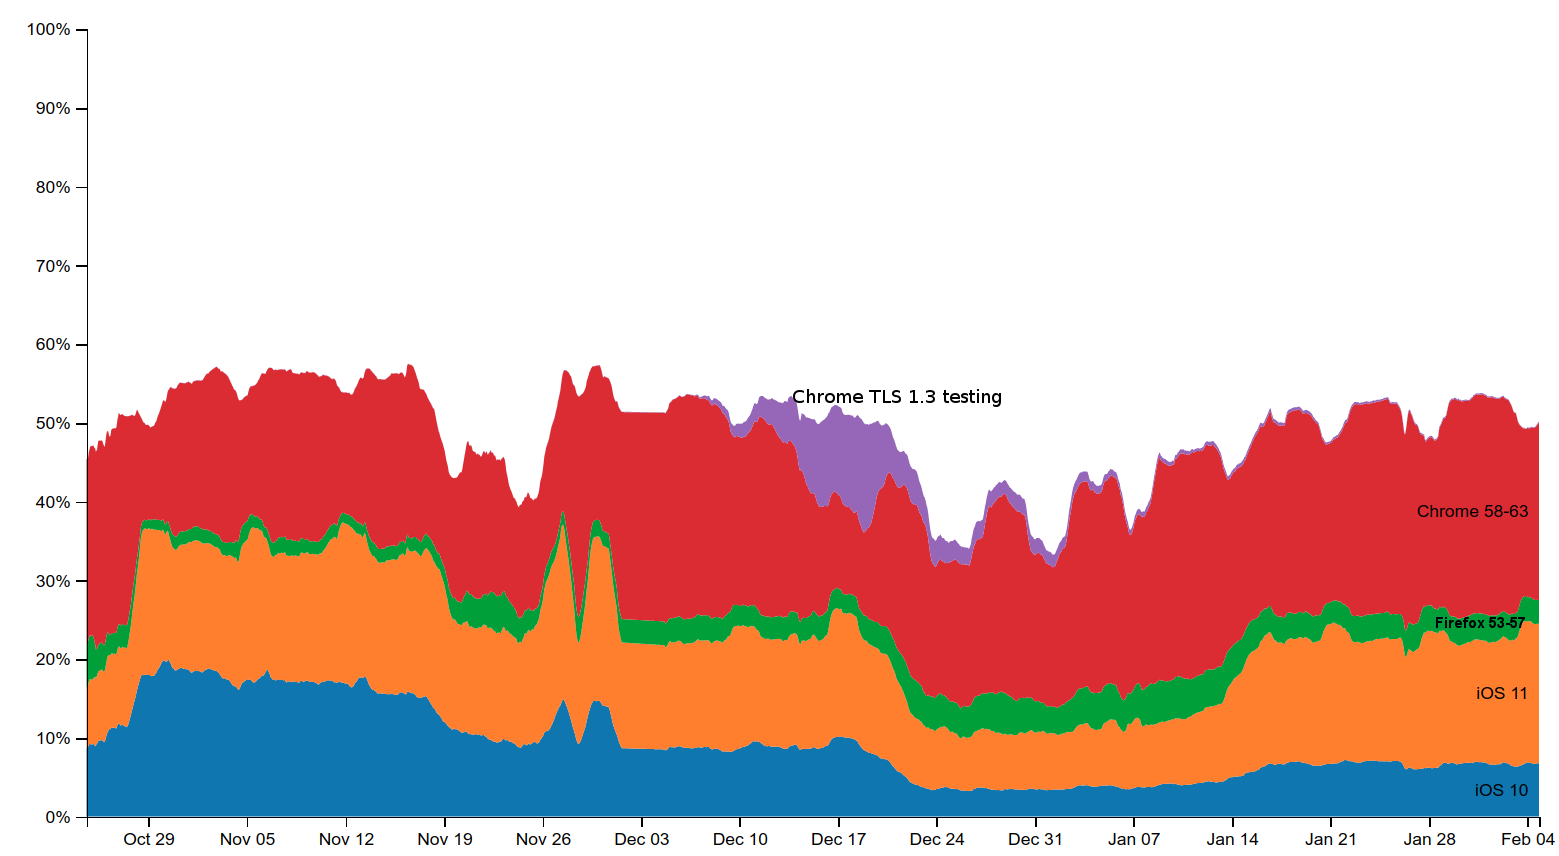
\includegraphics[width=0.9\linewidth,clip]{figures/browsers.png}
    \caption{\textbf{Popular Clients}\,---\, %
            Stacked graph showing the percent of connections (averaged over 24 hours) of popular clients,
            including recent versions of Chrome, Firefox, and versions
    of Apple iOS.  These popular clients make up roughly half of all seen connections.
    Also visible is the brief experiment Google Chrome performed in December where clients sent
    TLS~1.3 ClientHellos. 
    }
    \label{fig:browsers}
\end{figure}
}


\newcommand{\FigWhitelistChurn}{
	\begin{figure}[ht]
		\centering
		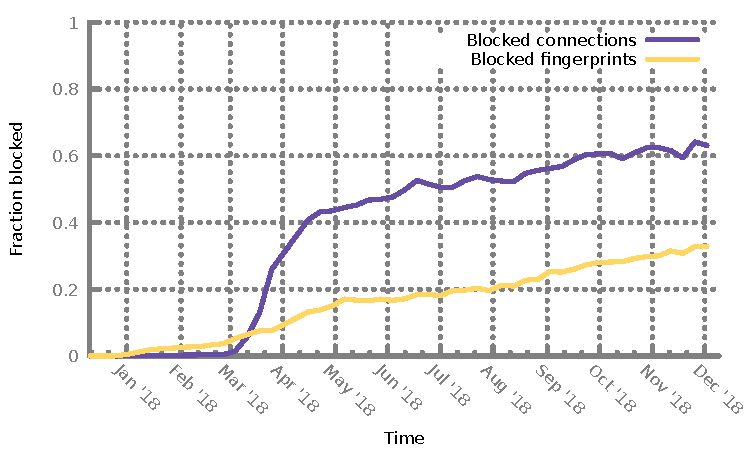
\includegraphics[width=0.9\linewidth,clip]{figures/churn.pdf}
		\caption{\textbf{Fingerprint turnover}\,---\,
            Shows fraction of connections/fingerprints not seen during the
            first week. This roughly models the fraction that censor would overblock,
            if they took a static fingerprint snapshot and whitelisted it.
        }
	\label{fig:wl-churn}
    \end{figure}
}


\newcommand{\FigTLS}{
\begin{figure}[ht]
    \centering
    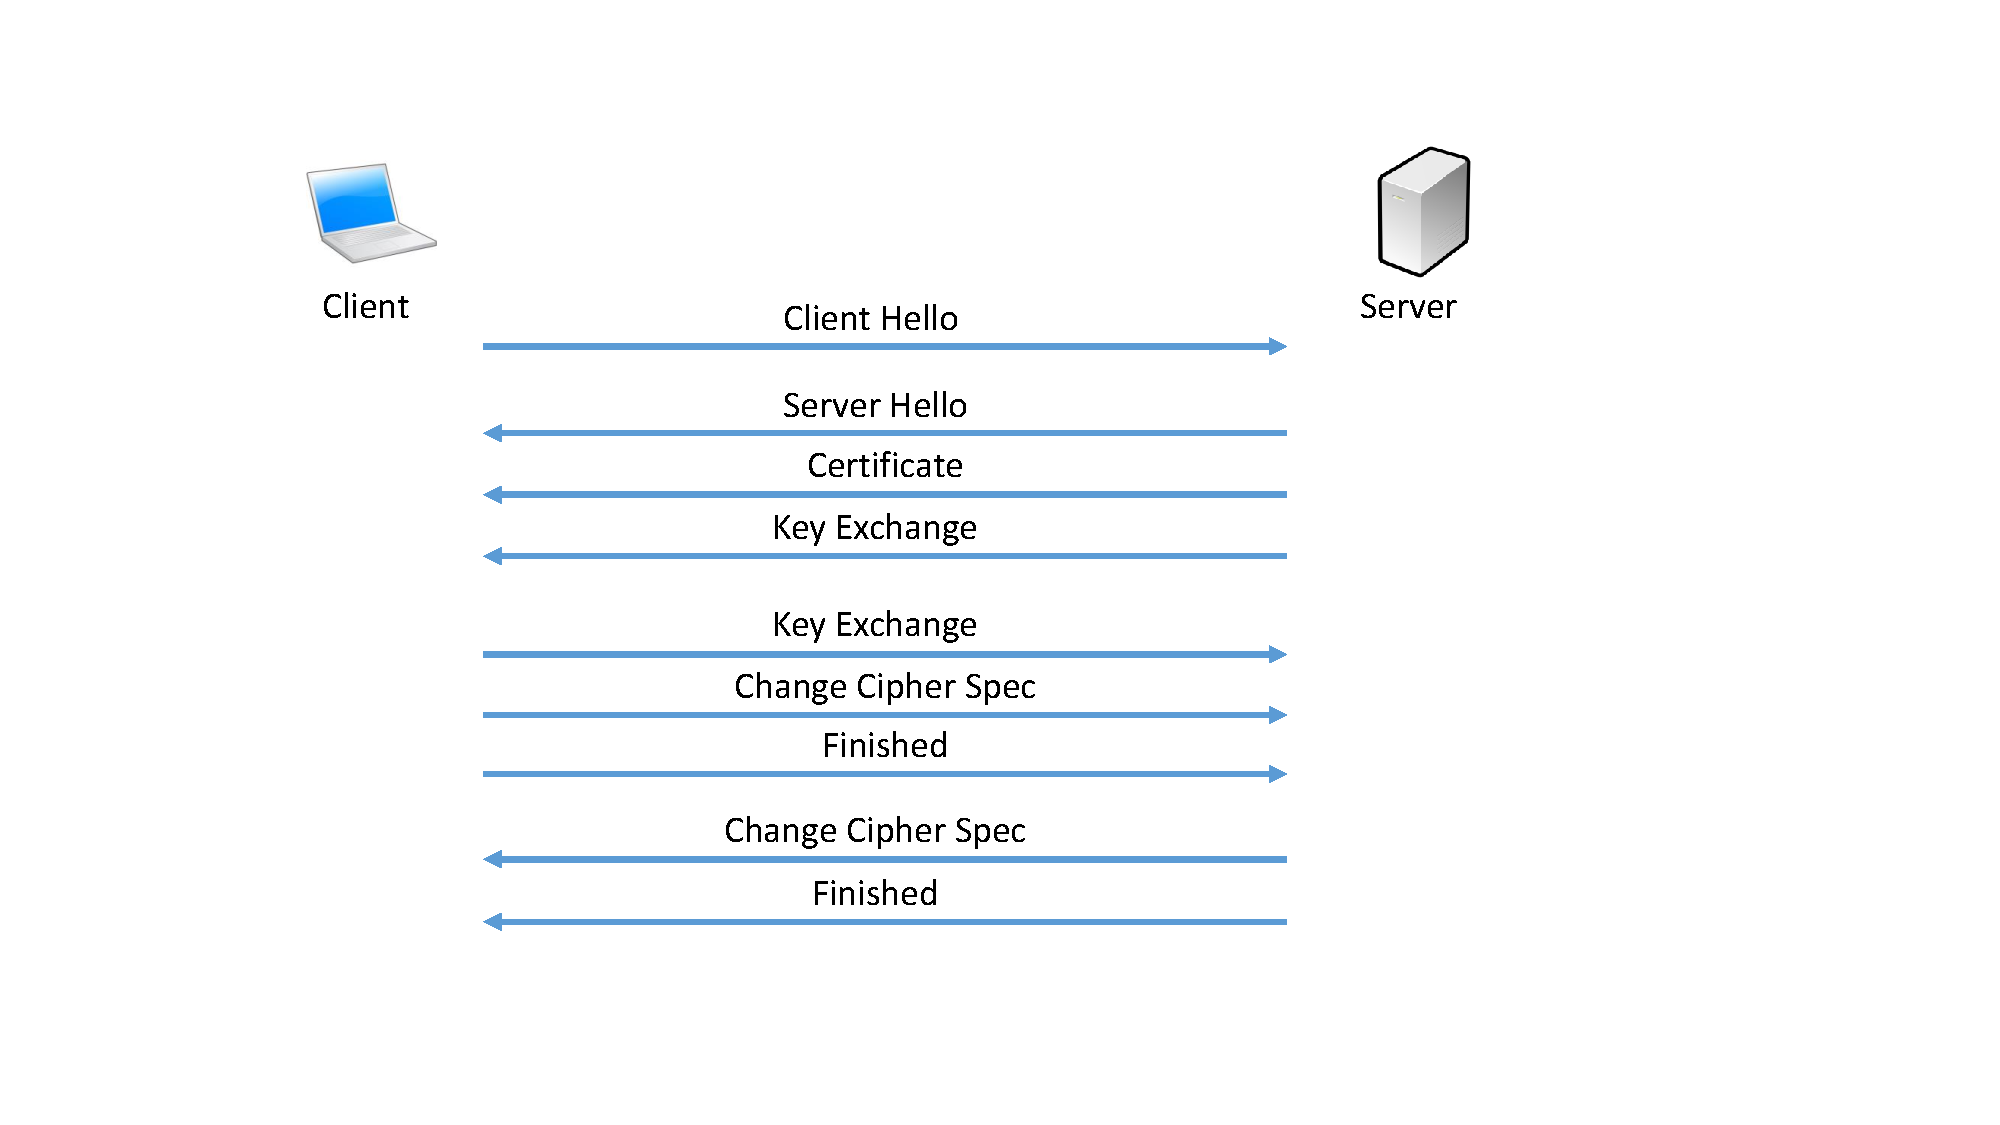
\includegraphics[width=0.9\linewidth,clip]{figures/tls.pdf}
    \caption{\textbf{TLS Handshake}\,---\, %
    The TLS handshake contains several messages sent unencrypted, including the Client Hello.
    This allows us to fingerprint client implementations by the features and parameters they send
    in this initial message.
}
    \label{fig:tls-handshake}
\end{figure}
}

\newcommand{\FigArch}{
\begin{figure*}[ht]
    \centering
    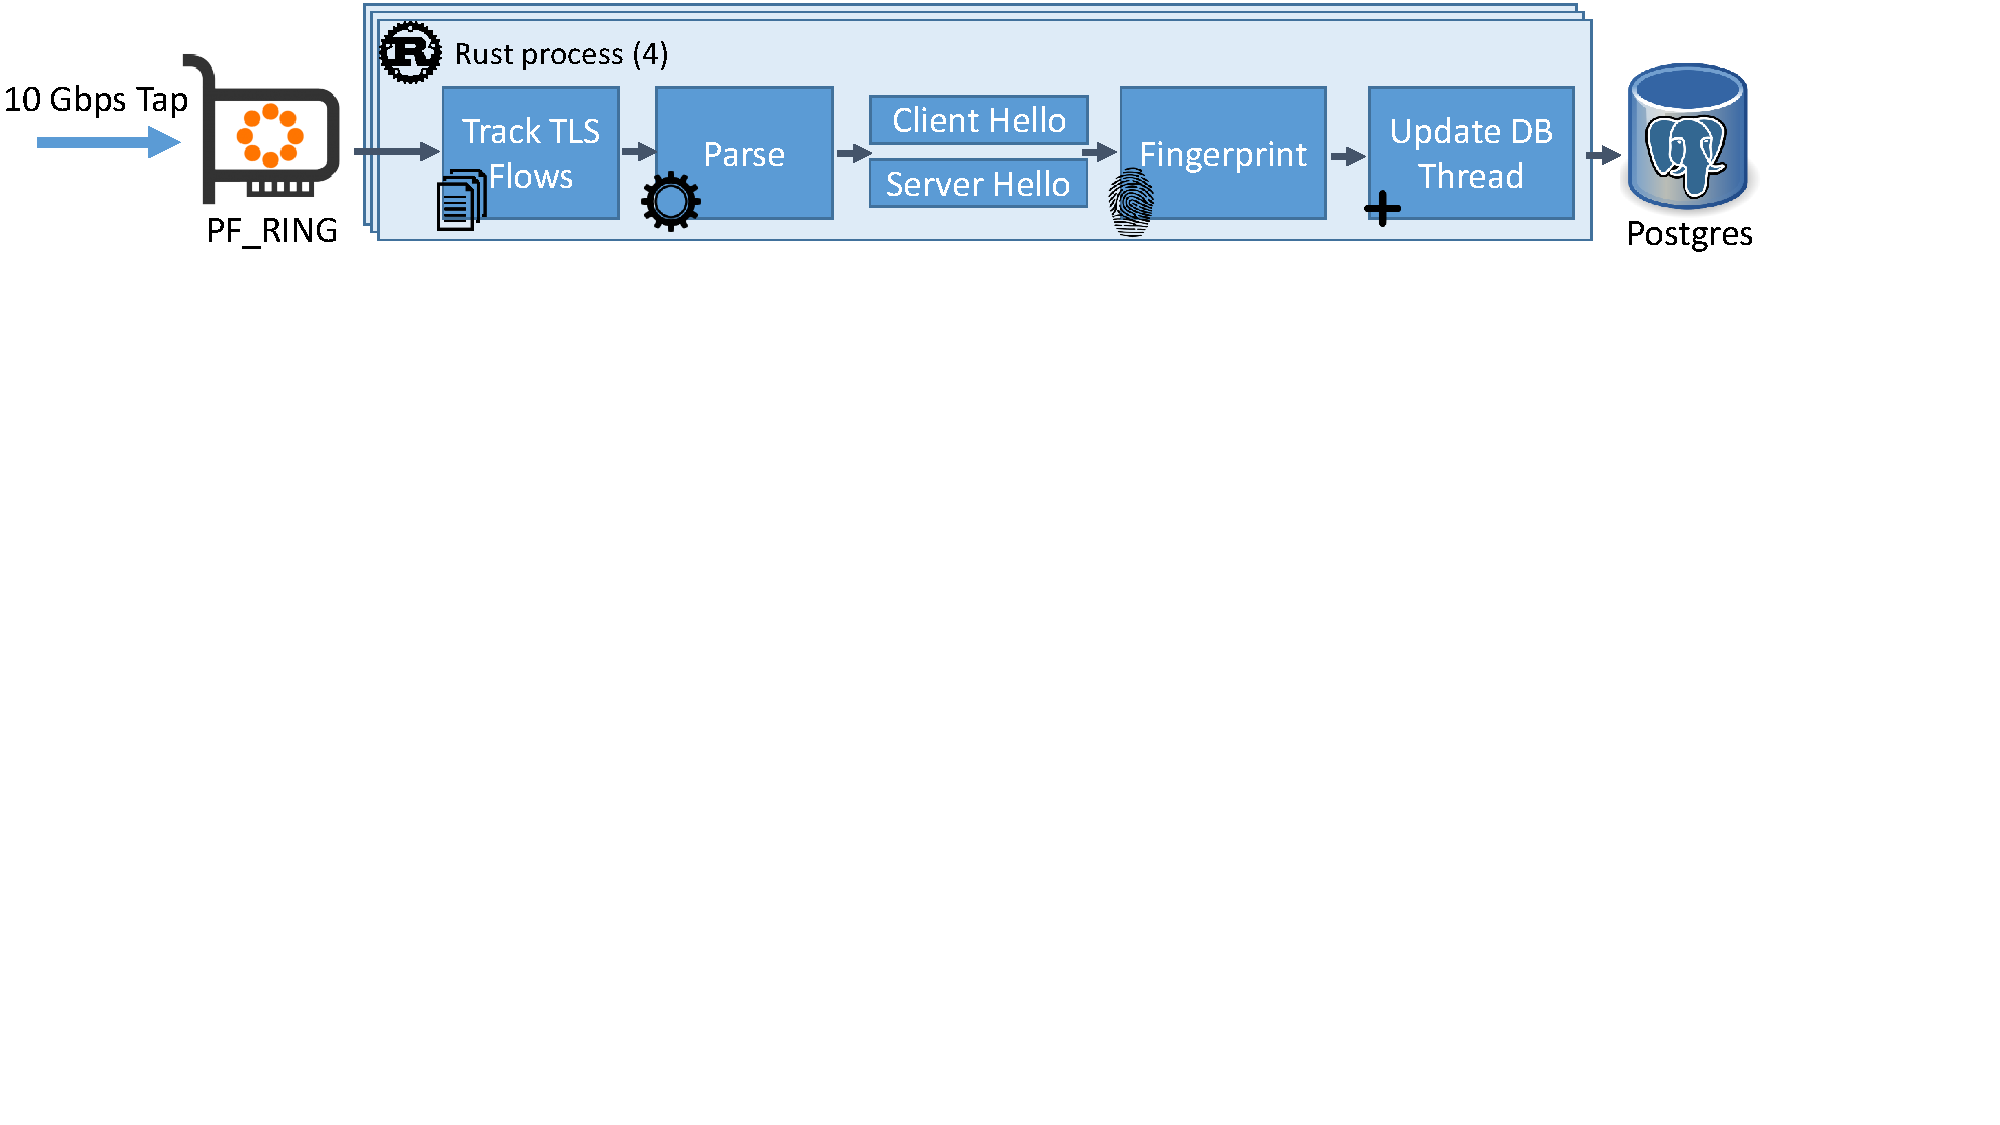
\includegraphics[width=0.9\linewidth,clip]{figures/architecture.pdf}
    \caption{\textbf{Collection Architecture}\,---\, %
    We implemented our 10~Gbps collection infrastructure using PF\_RING and 1400 lines
    of Rust, utilizing 4 processes. TLS client and ServerHello fingerprints and 
    counts
    were aggregated and periodically written to a PostgreSQL database in a separate thread
    to avoid blocking the main packet parsing loop.}
    \label{fig:arch}
\end{figure*}
}

\newcommand{\FigDiff}{
\begin{figure}[ht]
    \centering
    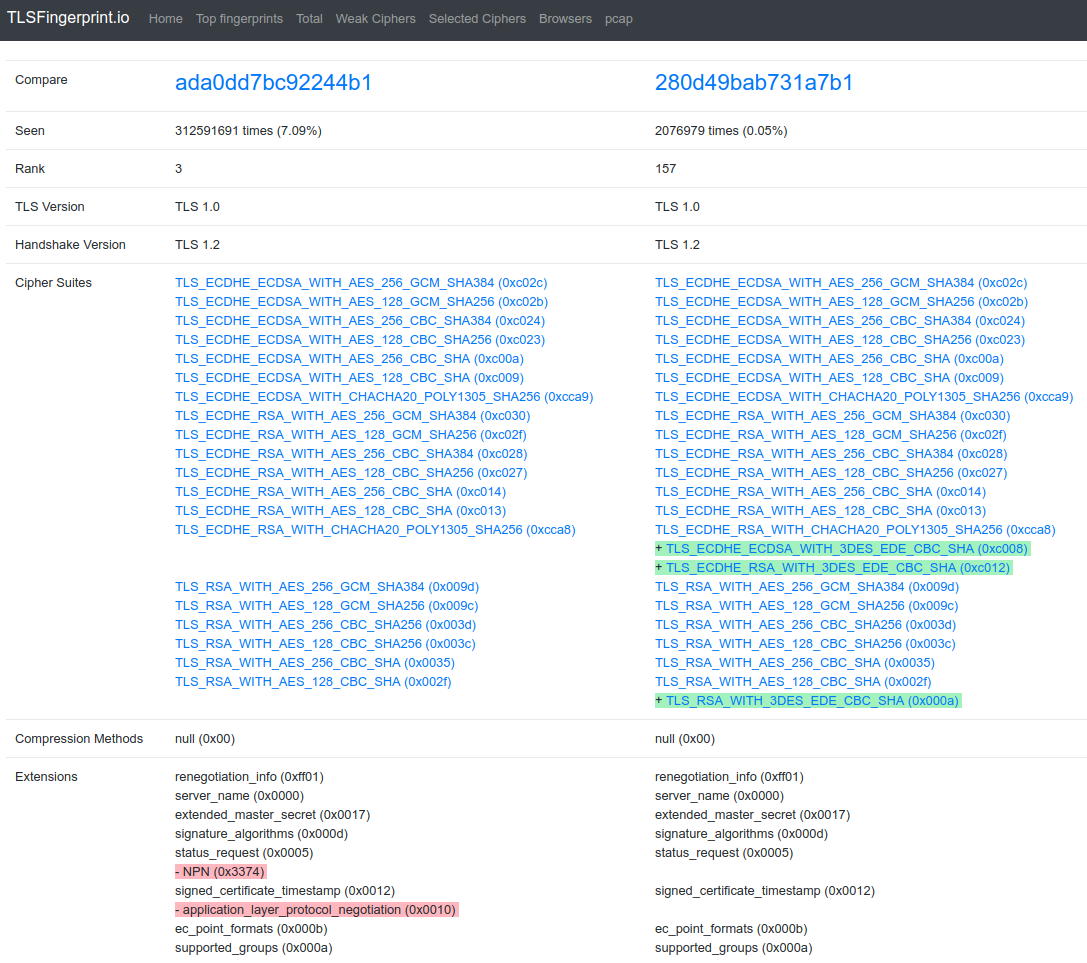
\includegraphics[width=0.9\linewidth,clip]{figures/compare.png}
    \caption{\textbf{Fingerprint comparison}\,---\,Our website supports
            comparing fingerprints and locating similar fingerprints based off
            of a Levenshtein distance over the various ClientHello parts. We
            can then easily show a diff between fingerprints, allowing them to
            be grouped with similar fingerprints generated by the same
    implementation.}
    \label{fig:diff}
\end{figure}
}

\newcommand{\FigTotal}{
\begin{figure}[ht]
    \centering
    \includegraphics[width=0.9\linewidth,clip]{figures/total.pdf}
    \caption{\textbf{Connections observed}\,---\,We collected 9 months of
            TLS connections on our 10~Gbps campus network, observing over 
            11~billion
            connections. Noticeable is
            the diurnal pattern of traffic, as well as a decrease in traffic on weekends
            and holiday breaks.}
    \label{fig:total}
\end{figure}
}

\newcommand{\FigUniqueFingerprints}{
\begin{figure}[ht]
    \centering
    \includegraphics[width=1\linewidth,clip]{figures/tot-uniq.pdf}
    \caption{\textbf{Total Unique Fingerprints}\,---\,The
            number of unique TLS ClientHello fingerprints observed rises
            slowly but steadily over time, reaching over 152,000 by
            May~2018. This rise is
            punctuated by short but rapid increases in the number of unique
            fingerprints, which we determined came
            from a small set of Internet scanners sending seemingly random
    ClientHello messages.}
    \label{fig:tot-uniq}
\end{figure}
}


\newcommand{\FigCDF}{
\begin{figure}[ht]
    \centering
    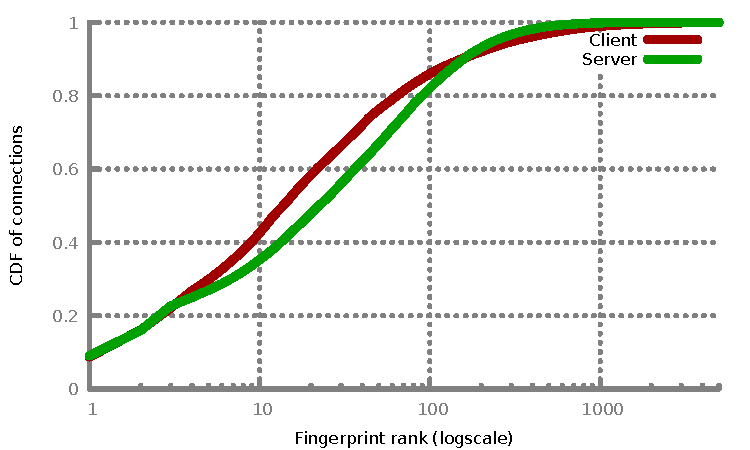
\includegraphics[width=0.9\linewidth,clip]{figures/fingerprints-cdf.pdf}
    \caption{\textbf{CDF of connections per fingerprint}\,---\,
            While we observed over 152,000 ClientHello fingerprints,
            most connections were comprised of a small number of fingerprints:
            over half the connections were of one of the top 12 fingerprints,
            and the top 3000 fingerprints make up 99.9\% of
    connections observed. For servers, only 4,700 fingerprints were observed,
    with half of the connections using one of the top 19 server fingerprints.}
    \label{fig:client-cdf}
\end{figure}
}

\newcommand{\FigServerCDF}{
\begin{figure}[ht]
    \centering
    \includegraphics[width=0.9\linewidth,clip]{figures/sfingerprints-cdf.pdf}
    \caption{\textbf{CDF of server fingerprints}\,---\,
            We observed 3,700 ServerHello fingerprints, and
            most connections were comprised of a small number of fingerprints,
            with top 19 fingerprints being used in over half the connections.
            This CDF is similar to ClientHello CDF, but has a much smaller tail.}
    \label{fig:server-cdf}
\end{figure}
}


\newcommand{\TabInvalid}{
\begin{table}
    \centering
    \scalebox{0.85}{
    \begin{tabular}{ l  c  c }
            \toprule
            & Fingerprints & \% Connections \\
            \hline

            % Updated Aug 7, 2018
            TLS 1.3 draft ciphers &  1002 & 10.626\%    \\
            Legacy ciphers &  82992 & 1.392\%   \\
            GOST ciphers &  95548 & 0.051\% \\
            Outdated SSL ciphers &  106439 & 0.097\%    \\
            Unknown ciphers & 137999 & 0.039\%  \\
            \textbf{Total non-standard ciphers} & \textbf{143060} & \textbf{12.106}\%  \\
            \hline
            TLS 1.3 draft extensions & 715 & 10.626\% \\
            Legacy Extensions & 441 & 0.154\% \\
            Extended Random & 340 & 1.445\% \\
            Unknown extensions & 367 & 0.899\% \\
            \textbf{Total non-standard extensions} & \textbf{1404} & \textbf{11.677}\% \\
            \toprule


        %Invalid ciphers &
            %% Updated: May 7, 2018
            %TLS 1.3 draft ciphers &  776 & 5.236\% \\
            %Legacy ciphers &  62289 & 1.482\% \\
            %GOST ciphers &  70336 & 0.011\% \\
            %Outdated SSL ciphers &  79467 & 0.053\% \\
            %Unknown ciphers & 102175 & 0.002\% \\
            %\textbf{Total non-standard ciphers} & \textbf{106506} & \textbf{6.762\%} \\
            %\hline
            %TLS 1.3 draft extensions & 488 & 5.235\% \\
            %Legacy Extensions & 423 & 0.166\% \\
            %Extended Random & 320 & 1.747\% \\
            %Unknown extensions & 262 & 0.906\% \\
            %\textbf{Total non-standard extensions} & \textbf{1119} & \textbf{6.309\%} \\
            %\toprule


            %Old, from february:
            %TLS 1.3 draft ciphers &  255 & 3.93\%  \\
            %Legacy ciphers &  34200 & 1.65\%   \\
            %GOST ciphers &  37993 & 0.006\% \\
            %Outdated SSL ciphers &  43065 & 0.053\% \\
            %Unknown ciphers & 54920 & 0.002\%   \\
            %\textbf{Total non-standard ciphers} & \textbf{58296} & \textbf{5.63\%}    \\

            %\hline
            %TLS 1.3 draft extensions & 261 & 3.93\% \\
            %Legacy Extensions & 356 & 0.17\%   \\
            %Extended Random & 264 & 3.93\% \\
            %Unknown extensions & 181 & 0.80\% \\
            %\textbf{Total non-standard extensions} & \textbf{775} & \textbf{4.90\%} \\
            %\toprule
    \end{tabular}
    }
    \caption{\textbf{Non-standard parameters}\,---\,
            Breakdown of the number of unique Client Hellos (fingerprints) and
            the share of connections they appear in that send non-standard cipher
            suites or extensions. While TLS~1.3 draft ciphers and extensions are
    the majority, we still find unknown ciphers and extensions in use.}
    \label{tab:invalid}
\end{table}
}

\newcommand{\TabWeak}{
\begin{table}
    \centering
    \begin{tabular}{ l  c  c }
            \toprule
            & Fingerprints & \% Connections \\
            \hline

            % Aug 2018:
            DES & 191459 & 0.90\% \\
            3DES & 236859 & 67.0\% \\
            EXPORT & 194418  & 0.66\% \\
            RC4 & 223900 & 8.19\% \\
            MD5 (Cipher) & 200608 &    7.15\% \\
            \hline
            MD5 (Sigalg) & 4385 & 0.74\% \\
            SHA1 (Sigalg) & 114615 & 97.6\% \\

            TLS\_FALLBACK & 787 & 0.03\% \\


            % May 2018
            %DES & 54727 & 0.92\% \\
            %3DES & 72405 & 61.7\% \\
            %EXPORT & 56543  & 0.67\% \\
            %RC4 & 64075 & 9.13\% \\
            %MD5 (Cipher) & 61050 &    7.92\% \\
 
            %MD5 (Sigalg) & 1686 & 0.70\% \\
            %SHA1 (Sigalg) & 43456 & 97.9\% \\

            %TLS\_FALLBACK & 571 & 0.03\% \\
            \toprule
    \end{tabular}
    \caption{\textbf{Weak ciphers}\,---\, We analyzed the percent of connections
            offering known weak cipher suites. We also include
            \texttt{TLS\_FALLBACK\_SCSV}, which indicates a client that
            is falling back to an earlier version than it supports due to the
            server not supporting the same version.}
    \label{tab:weak}
\end{table}
}

\newcommand{\TabPopularCiphers}{
\begin{table*}[ht]
    \centering
    % view-source:https://tlsfingerprint.io/top-ciphers/
    % Note: excludes fingerprints seen only once...
    \begin{tabular}{ l l c c }
            \toprule
            Rank & Cipher Suite & Fingerprints & \% Connections \\
            \hline
            1  & TLS\_ECDHE\_RSA\_WITH\_AES\_128\_CBC\_SHA & 27798   & 99.1\% \\
            2  & TLS\_ECDHE\_RSA\_WITH\_AES\_256\_CBC\_SHA & 26595   & 98.7\% \\
            3  & TLS\_RSA\_WITH\_AES\_128\_CBC\_SHA &   31014   &  94.4\% \\
            4  & TLS\_RSA\_WITH\_AES\_256\_CBC\_SHA &   30087   &  94.2\% \\
            5  & TLS\_ECDHE\_ECDSA\_WITH\_AES\_128\_GCM\_SHA256 &    27849  &  94.0\% \\
            6  & TLS\_ECDHE\_RSA\_WITH\_AES\_128\_GCM\_SHA256 &  24642   &  92.6\% \\
            7  & TLS\_ECDHE\_ECDSA\_WITH\_AES\_256\_GCM\_SHA384 &    25643 &  92.5\% \\
            8  & TLS\_ECDHE\_RSA\_WITH\_AES\_256\_GCM\_SHA384 &  21891   &  91.1\% \\
            9  & TLS\_RSA\_WITH\_AES\_128\_GCM\_SHA256 &    26130   &  84.6\% \\
            10 & TLS\_RSA\_WITH\_AES\_256\_GCM\_SHA384 &    23635   &  83.2\% \\
            \toprule
    \end{tabular}
    \caption{\textbf{Popular Cipher Suites}\,---\, Top ten popular cipher suites offered by clients,
                weighted by connections. Small handful of cipher suites appear to be
                supported by the vast majority of clients in use.}
    \label{tab:popularciphers}
\end{table*}
}

\newcommand{\TabTopFingerprints}{
\begin{table}[ht]
    \centering
    % view-source:https://tlsfingerprint.io/top-ciphers/
    % Note: excludes fingerprints seen only once...
        \textbf{August 2018}
    \begin{tabular}{ r l c }
            \toprule
            Rank & Client & \% Connections \\
            \hline
            1  & Chrome 65-68 & 16.51\%   \\  % 177
            2  & iOS 11/macOS 10.13 Safari & 5.95\%        \\  % 77
            3  & MS Office 2016 (including Outlook) &  5.34\% \\ % 338
            4  & Chrome 65-68 (with padding) &  4.62\% \\   % 177
            5  & Edge 15-18, IE 11 &  4.05\% \\    % 338
            6  & Firefox 59-61 (with padding) &  3.62\% \\  % 48
            7  & Safari 11.1 on Mac OS X &  2.82\% \\   % 77
            8  & iOS 10/macOS 10.12 Safari & 2.49\% \\ % 51
            9  & iOS 11/macOS 10.13 Safari (with padding) & 2.42\% \\ % 77
            10 & Firefox 59-61 & 2.22\% \\ % 48
            \toprule
    \end{tabular}
        \\
        \textbf{December 2018} \\
    \begin{tabular}{ r l c }
            \toprule
            Rank & Client & \% Connections \\
            \hline
            1    & Chrome 70 (with padding) & 8.49\% \\
            2    & iOS 12/macOS 10.14 Safari & 7.55\% \\
            3    & iOS 12/macOS 10.14 Safari (without ALPN) & 4.15\% \\
            4    & Chrome 70 & 4.10\% \\
            5    & iOS 12/macOS 10.14 Safari (with padding) & 4.09\% \\
            6    & Edge 15-18, IE 11 & 3.27\% \\
            7    & MS Office 2016 (including Outlook) & 3.01\% \\ 
            8    & iOS 10/macOS 10.12 Safari & 2.72\% \\
            9    & iOS 11/macOS 10.13 Safari & 2.68\% \\
            10   & Chrome 71 (with padding) & 2.48\% \\ % released Dec 4th
            \toprule
    \end{tabular}
    \caption{\textbf{Top 10 Implementations.}\,---\, Most frequently seen fingerprints in our
        dataset and the implementations that generate them, for a week in August and December~2018.
        Despite being only 4 months apart,
        top 10 fingerprints changed substantially, as
        new browser releases quickly take the place of older versions.}

        %These implementations are responsible for generating just over half the connections we see.
    %Rank and amount of connections are for one week of measurements in early August 2018.
    %Fingerprints with and without padding are otherwise identical: the padding extension is commonly
    %added by TLS stacks to work around bugs in deployed middleboxes.}
    \label{tab:toptenfingerprints}
\end{table}
}

\newcommand{\TabTopFingerprintsDecember}{
\begin{table}[ht]
    \centering
    % view-source:https://tlsfingerprint.io/top-ciphers/
    % Note: excludes fingerprints seen only once...
    \begin{tabular}{ r l c }
            \toprule
            Rank & Client & \% Connections \\
            \hline
            1    & Chrome 70 with padding & 8.49\% \\
            2    & iOS 12/macOS 10.14 Safari & 7.55\% \\
            3    & iOS 12/macOS 10.14 Safari without ALPN & 4.15\% \\
            4    & Chrome 70 & 4.10\% \\
            5    & iOS 12/macOS 10.14 Safari with padding & 4.09\% \\
            6    & Edge 15-18, IE 10 on Windows 10 & 3.27\% \\
            7    & MS Office 2016 & 3.01\% \\ 
            8    & iOS 10/macOS 10.12 Safari & 2.72\% \\
            9    & iOS 11/macOS 10.13 Safari & 2.68\% \\
            10   & Chrome 71 with padding & 2.48\% \\ % released Dec 4th
            \toprule
    \end{tabular}
    \caption{\textbf{Top 10 Implementations. December, 2018}\,---\, Most frequently seen fingerprints in our
        dataset and the implementations that generate them.
    Rank and amount of connections are for one week of measurements in between December 6th and 13th 2018:
    Chrome 71 was released on December 4th and is gradually replacing Chrome 70.
    Note that Chrome started to generate padded version more often than non-padded:
    padding is included when ClientHello is between 256 and 512 bytes long
    to work around bugs in deployed middleboxes,
    and addition of new TLS 1.3 extensions with new data made ClientHellos
    go over 256 bytes more often.
    }
    \label{tab:toptenfingerprints}
\end{table}
}

\newcommand{\TabSelectedCiphers}{
\begin{table*}[ht]
    \centering
    % view-source:https://tlsfingerprint.io/server-ciphers
    \tabcolsep=0.11cm
    \scalebox{0.9}{
    \begin{tabular}{l c c c }
            \toprule
        Cipher Suite & Client Fingerprints & Server Fingerprints & \% Connections \\
            \hline

            TLS\_ECDHE\_RSA\_WITH\_AES\_128\_GCM\_SHA256 & 5137 & 438 & 50.71 \\

            TLS\_ECDHE\_RSA\_WITH\_AES\_256\_GCM\_SHA384 & 3054 & 268 & 19.29 \\

            TLS\_ECDHE\_ECDSA\_WITH\_AES\_128\_GCM\_SHA256 & 1656 & 264 & 13.30 \\

            TLS\_ECDHE\_ECDSA\_WITH\_AES\_256\_GCM\_SHA384 & 765 & 115 & 2.45 \\

            TLS\_RSA\_WITH\_AES\_256\_CBC\_SHA & 1300 & 123 & 1.60 \\

            TLS\_RSA\_WITH\_AES\_256\_CBC\_SHA256 & 2711 & 45 & 1.56 \\

            TLS\_RSA\_WITH\_AES\_128\_CBC\_SHA & 2688 & 134 & 1.49 \\

            TLS\_ECDHE\_RSA\_WITH\_CHACHA20\_POLY1305\_SHA256 & 333 & 170 & 1.38 \\

            TLS\_RSA\_WITH\_AES\_256\_GCM\_SHA384 & 855 & 56 & 1.38 \\

            TLS\_ECDHE\_RSA\_WITH\_AES\_256\_CBC\_SHA384 & 1023 & 121 & 1.31 \\

            % Top 10: 94.40% of connections total
            \toprule
    \end{tabular}
    }
    \caption{\textbf{Server Hello Selected Ciphers}\,---\,The top ten most common ciphers selected accounted for
            over 94\% of connections with all connections choosing one of only 47 cipher suites,
            showing significantly less server diversity than client fingerprints, which had over 6600 unique sets
            of cipher suites sent in 21,000 ClientHello fingerprints seen more 
            than once.}
    \label{tab:selected}
\end{table*}
}


\newcommand{\TabSelectedALPN}{
\begin{table}
    % From https://tlsfingerprint.io/alpn
    \centering
    \tabcolsep=0.11cm
    \scalebox{0.9} {
    \begin{tabular}{r c c}
            \toprule

            % May 2018
            ALPN & Fingerprints & \% Connections \\
            \hline
            \emph{None} & 156247 & 58.4\% \\
            h2 & 22562 & 22.0\% \\
            http/1.1 & 36292 & 19.3\% \\
            apns-pack-v1:4096:4096 & 3 & 0.2\% \\
            spdy/3.1 & 1313 & 0.1\% \\


            % February 2018:
            %Selected ALPN & Fingerprints & \% Connections \\
            %\hline
            %\emph{None} & 72681 & 58.38\% \\
            %    h2 & 13101 & 22.36\% \\
            %    http/1.1 & 21040 & 18.92\% \\
            %    spdy/3.1 & 902 & 0.18\% \\
            %    apns-pack-v1:4096:4096 & 3 & 0.16\% \\
            \toprule
    \end{tabular}
    }
    \caption{\textbf{Selected ALPN}\,---\, Top five most commonly selected ALPN. HTTP/2 outranks
            explicit HTTP/1.1 support, though likely the majority of connections that
            provided no ALPN (58\%) defaulted to HTTP/1.1. Despite only having 3 distinct fingerprints,
            Apple's push notification service (APNS) accounts for 0.16\% of all connections.
    }
    \label{tab:selectedALPN}
\end{table}
}


\newcommand{\TabTools}{
	\begin{table}
		\centering
		\tabcolsep=0.11cm
		\scalebox{0.9} {
			\begin{tabular}{l r l l}
				\toprule
                    Tool & Version/Date & Rank [all time] & \% Connections \\
				\hline
                    \textbf{Psiphon} & Jan 2018 & 1 & 8.76\% \\
                    & & 9 & 2.42\% \\
                    & & 62 & 0.25\% \\
                    & & 198 & \textcolor{red}{0.04\%} \\
                    & & 203 & \textcolor{red}{0.04\%} \\
                    & & 500 & \textcolor{red}{0.01\%} \\
                    & & 2190 & \textcolor{red}{0.0002\%} \\
                    & & 14397 & \textcolor{red}{0.0000\%} \\ % < 0.0001%
                    & & 16814 & \textcolor{red}{0.0000\%} \\ % < 0.0001
%\hline
                    \textbf{Outline} & May 2018 & 1 & 8.76\% \\
%\hline
                    \textbf{meek} & TBB 7.5 & 42 & 0.50\% \\
%\hline
                    \textbf{Snowflake} & April 2018 & 1378 & \textcolor{red}{0.0008\%} \\
%\hline
                    \textbf{Lantern} & 4.6.13 & 1867 & \textcolor{red}{0.0003\%} \\
%\hline
                    \textbf{TapDance} & May 2018 & random & - \\
%\hline
                    \textbf{Signal} & 4.19.3 & 11468 & \textcolor{red}{0.0000\%} \\
                    &   & 12982 & \textcolor{red}{0.0000\%} \\
				\toprule
			\end{tabular}
		}
		\caption{\textbf{Tool Fingerprintability}\,---\, Summary of all TLS
		fingerprints generated by censorship circumvention tools and their
            rank and percent of connections seen in our dataset as of early August 2018.
            Highlighted in red are fingerprints seen in relatively few ($<$ 0.1\%)
            connections, putting them at risk of blocking by a censor.
		}
		\label{tab:tools}
	\end{table}
}

\newcommand{\TabPopularALPN}{
\begin{table}
    % From https://tlsfingerprint.io/alpn
    \centering
    \tabcolsep=0.11cm
    \scalebox{0.9} {
    \begin{tabular}{r c c}
            \toprule


        % Updated Aug 7, 2018
        ALPN & Fingerprints & \% Connections \\
        \hline
                http/1.1 & 8078 & 70.3\% \\
                h2 & 5200 & 64.1\% \\
                spdy/3.1 & 2421 & 23.2\% \\
                spdy/3 & 1006 & 22.5\% \\
                h2-14 & 755 & 19.9\% \\
                h2-15 & 460 & 19.9\% \\
                h2-16 & 472 & 19.9\% \\
                h2-fb & 99 & 0.3\% \\
                apns-pack-v1 & 2 & 0.1\% \\
                apns-security-v3 & 2 & 0.1\% \\

        % May 2018
        %http/1.1 & 7032 & 70.8\% \\
        %h2 & 4534 & 64.6\% \\
        %spdy/3.1 & 2219 & 25.0\% \\
        %spdy/3 & 901 & 24.3\% \\
        %h2-14 & 664 & 21.5\% \\
        %h2-15 & 389 & 21.4\% \\
        %h2-16 & 399 & 21.4\% \\
        %h2-fb & 85 & 0.3\% \\
        %apns-pack-v1 & 2 & 0.1\% \\
        %apns-security-v3 & 2 & 0.1\% \\


            % February 2018:
            %ALPN & Fingerprints & \% Connections \\
            %    \hline
            %        http/1.1 & 5807 & 70.7\% \\
            %        h2 & 3748 & 64.4\% \\
            %        spdy/3.1 & 1971 & 26.0\% \\
            %        spdy/3 & 776 & 25.2\% \\
            %        h2-14 & 549 & 22.2\% \\
            %        h2-15 & 298 & 22.1\% \\
            %        h2-16 & 310 & 22.1\% \\
            %        h2-fb & 53 & 0.3\% \\
            %        apns-pack-v1 & 2 & 0.1\% \\
            %        apns-security-v3 & 2 & 0.1\% \\
            \toprule
    \end{tabular}
    }
    \caption{\textbf{Popular ALPN}\,---\, Top most commonly supported ALPNs. In total, there
            were 526 unique ALPN values sent by clients, though the vast majority were invalid random values.
            Prominent in this data is support for HTTP/2 (h2) and its draft versions,
            Google's \texttt{spdy} protocol, and Apple's Push Notification Service (APNS) protocol.
    }
    \label{tab:popularALPN}
\end{table}
}

\newcommand{\FigTopNoSNI}{
    \begin{figure}[ht]
        \centering
    \includegraphics[width=0.9\linewidth,clip]{figures/sniless-cdf.pdf}
    \caption{\textbf{CDF of connections sending no SNI}\,---\, %
        We observed 1.4\% of connections did not send the server name indication (SNI)
        extension, with the majority coming from just 10 fingerprints. This suggests a censor
        could easily block circumvention tools that do not send SNIs, with either a small
        amount of collateral overblocking or minimal whitelisted exceptions.}
    \label{fig:sniless-cdf}
    \end{figure}
}

\newcommand{\TabTopNoSNI}{
	\begin{table}[ht]
		% From https://tlsfingerprint.io/alpn
		\centering
		\tabcolsep=0.11cm
		\scalebox{0.9} {
			\begin{tabular}{r c}
				\toprule
				Rank & Connections [all time] \\ %& Rank [all time] & Rank 
				%[25 April 
				%- 2 May 2018] \\
				\hline
1 & 0.1956 \% \\  %& 68 & 77 \\
2 & 0.0857 \% \\  %& 111 & 137 \\
3 & 0.0745 \% \\  %& 125 & 314 \\
4 & 0.0560 \% \\  %& 140 & - \\
5 & 0.0540 \% \\  %& 143 & 152 \\
6 & 0.0499 \% \\  %& 149 & 153 \\
7 & 0.0478 \% \\  %& 160 & 143 \\
8 & 0.0476 \% \\  %& 163 & 164 \\
9 & 0.0471 \% \\  %& 164 & 227 \\
10 & 0.0450 \%\\  % & 167 & 948 \\

%8577568175451810252  
%-6423993798557871268 
%1380591653976699571  
%-2791419216777605277 
%-5231413793168069546 
%417772208000436940   
%502795999810062699   
%3080265117687502513  
%-4261455803793459001 
%-3124589779202159765 
%-2022210942072690627 & 0.0438 \% & 169 & 161 \\
				\toprule
			\end{tabular}
		}
		\caption{\textbf{Top fingerprints that lack SNI}\,---\,
            TODO: this would be better as a CDF...
			Top ten popular fingerprints, that lack SNI,
			weighted by connections.
            %and their relative popularity as of May 2, 2018.
            In total, only TK\% of connections sent no SNI, suggesting that it
            would not cause sigificant collateral damage for a censor to block
            TLS connections that do not send this extension.
			%that they are used by bots, including top 1, 3 and 4 SNI-less
			%fingerprints of all time.
		}
		\label{tab:topNoSNI}
	\end{table}
}

\newcommand{\TabExtensions}{
    \begin{table}[ht]
        \centering
            \begin{tabular}{r l}
                \toprule
                Extension & Conns \\
                \hline
                    \textbf{supported\_groups} & 99.4\% \\
                    server\_name & 99.3\% \\
                    \textbf{signature\_algorithms} & 97.8\% \\
                    \textbf{ec\_point\_formats} & 96.9\% \\
                    extended\_master\_secret & 86.8\% \\
                    status\_request & 85.7\% \\
                    renegotiation\_info & 81.9\% \\
                    \textbf{ALPN} & 71.9\% \\
                    signed\_certificate\_timestamp & 66.9\% \\
                    SessionTicket & 56.0\% \\
                    padding & 32.3\% \\
                \toprule
            \end{tabular}
            \begin{tabular}{r l}
                \toprule
                Extension & Conns \\
                \hline
                    GREASE & 30.2\% \\
                    \textbf{psk\_key\_exchange\_modes}* & 28.7\% \\
                    \textbf{supported\_versions}* & 28.7\% \\
                    \textbf{key\_share}* & 28.6\% \\
                    NPN & 27.3\% \\
                    \textbf{compressed\_certificate}* & 24.8\% \\
                    ChannelID & 20.5\% \\
                    heartbeat & 5.0\% \\
                    token\_binding & 3.9\% \\
                    pre\_shared\_key* & 3.1\% \\
                    \textbf{record\_size\_limit} & 2.5\% \\
                \toprule
                \end{tabular}
            \caption{\textbf{Top Extensions}\,---\,
            While we include the presence and order of all extensions in our fingerprint,
            \textbf{Bold} denotes extensions whose data we additionally parse and include in our fingerprint;
            * marks extensions new in TLS~1.3.
            %Data shown for a week between December 5th and 12th, 2018.
            }
            \label{tab:extensions}
        \end{table}
}


%\fancyhf{} % Remove fancy page headers 
%\fancyhead[C]{Paper \#XXX} % TODO: replace 9999 with your paper number
%\fancyfoot[C]{\thepage}

%\setcopyright{none} % No copyright notice required for submissions
%\acmConference[Anonymous Submission to ACM CCS 2018]{ACM Conference on Computer and Communications Security}{Due 08 May 2018}{Toronto, Canada}
%\acmYear{2018}

%\settopmatter{printacmref=false, printccs=true, printfolios=true} % We want page numbers on submissions

%%\ccsPaper{9999} % TODO: replace with your paper number once obtained



\begin{document}
\title{The use of TLS in Censorship Circumvention}
\author{
        \authorblockN{Sergey Frolov}
        \authorblockA{University of Colorado Boulder\\
                    sergey.frolov@colorado.edu}
        \and
        \authorblockN{Eric Wustrow}
        \IEEEauthorblockA{University of Colorado Boulder \\
            ewust@colorado.edu}
}

%\IEEEoverridecommandlockouts
%\makeatletter\def\@IEEEpubidpullup{9\baselineskip}\makeatother
%\IEEEpubid{\parbox{\columnwidth}{Permission to freely reproduce all or part
%    of this paper for noncommercial purposes is granted provided that
%    copies bear this notice and the full citation on the first
%    page. Reproduction for commercial purposes is strictly prohibited
%    without the prior written consent of the Internet Society, the
%    first-named author (for reproduction of an entire paper only), and
%    the author's employer if the paper was prepared within the scope
%    of employment.
%}
\IEEEoverridecommandlockouts
\makeatletter\def\@IEEEpubidpullup{6.5\baselineskip}\makeatother
\IEEEpubid{\parbox{\columnwidth}{
    Network and Distributed Systems Security (NDSS) Symposium 2019\\
    24-27 February 2019, San Diego, CA, USA\\
    ISBN 1-891562-55-X\\
    https://dx.doi.org/10.14722/ndss.2019.23511\\
    www.ndss-symposium.org
}
\hspace{\columnsep}\makebox[\columnwidth]{}}



\maketitle

% todo: "Although we collected over 110,000 fingerprints" "While we observed over 75,000 Client Hello fingerprints"
\begin{abstract}

TLS, the Transport Layer Security protocol, has quickly become
the most popular protocol on the Internet, already used to load over 70\% of
web pages in Mozilla Firefox. Due to its ubiquity, TLS is also a popular
protocol for censorship circumvention tools, including Tor and Signal, among others.
%why just those? maybe add TapDance and Lantern?
% People have heard of these tools. 

However, the wide range of features supported in TLS makes it possible to
distinguish implementations from one another by what set of cipher suites,
elliptic curves, signature algorithms, and other extensions they support.
Already, censors have used deep packet inspection (DPI) to identify and
block popular circumvention tools based on the fingerprint of their TLS 
implementation.

In response, many circumvention tools have attempted to mimic popular TLS
implementations such as browsers, but this technique has several challenges.
First, it is burdensome to keep up with the rapidly-changing browser
TLS implementations, and know what fingerprints would be good candidates to mimic.
Second, TLS implementations can be difficult to mimic correctly, as
they offer many features that may not be supported by the relatively lightweight
libraries used in typical circumvention tools.
Finally, dependency changes and updates to the underlying libraries can silently
impact what an application's TLS fingerprint looks like, making it difficult for
tool maintainers to keep up.

In this paper, we collect and analyze real-world TLS traffic from over
11.8~billion TLS connections over 9 months to identify a wide range of TLS client
implementations actually used on the Internet. We use our data to analyze TLS
implementations of several popular censorship circumvention tools, including
Lantern, Psiphon, Signal, Outline, TapDance, and Tor (Snowflake and meek pluggable transports).
We find that the many of these tools use TLS configurations
that are easily distinguishable from the real-world traffic they attempt
to mimic, even when these tools have put effort into parroting popular TLS
implementations.

To address this problem, we have developed a library, uTLS, that enables tool
maintainers to \emph{automatically} mimic other popular TLS implementations. Using our
real-world traffic dataset, we observe many popular TLS implementations we are able to
correctly mimic with uTLS, and we describe ways our tool can more flexibly adapt
to the dynamic TLS ecosystem with minimal manual effort.

%To enable this study, we collect TLS packets from a 10~Gbps campus network and
%process them in real-time to extract a \emph{TLS fingerprint} for each
%connection, allowing us to group messages generated by the same implementation
%together. So far, we have recovered fingerprints from over 9.1~billion TLS 
%connections over the
%course of 5 months from real-world users. In addition to the results presented
%herein, we release a tool that allows others to explore our live data via a
%website: \url{https://tlsfingerprint.io}.
%
%In addition, to allow and encourage further research to utilize this fountain of
%information, we release a tool to explore our live data via a
%website: \url{https://tlsfingerprint.io}.
\end{abstract}


%\maketitle

\section{Introduction}

The Transport Layer Security (TLS) protocol is quickly becoming the most popular
protocol on the Internet, securing network communication from interference and
eavesdropping. Already, 70\% of page loads by Firefox users
make use of TLS~\cite{firefox-tls-adoption},
and adoption continues to grow
as more websites, services, and applications switch to TLS.

%Censors can easily identify and block custom protocols,
%which is why circumvention tools have turned to using existing standard
%protocols, tunneling through or mimicking popular applications,
%or looking random.
%Mimicking popular applications, such as Skype, was shown to be
%fundamentally flawed due to difficulty of enumerating potential application
%layer distinguishers~\cite{houmansadr2013parrot}.
%Tunneling via popular application is a very solid approach,
%but bundling another application and keeping it updated might be expensive
%in terms of memory, RAM (proxies on iOS have extremely low memory limit of 15 
%MiB), and in terms of effort,
%especially when original application does not provide needed API for such
%tunneling out of the box and requires patching.
%Random protocol is fingerprint in itself,
%and could be blocked as well.

Given the prevalence of TLS, it is commonly used by circumvention tools to evade
Internet censorship. Because censors can easily identify and block custom
protocols~\cite{houmansadr2013parrot}, circumvention tools have turned to using
existing protocols. TLS offers a convenient choice for these tools, providing
plenty of legitimate cover traffic from web browsers and other TLS user,
protection of content from eavesdroppers, and several libraries to choose from
that support it.

However, simply using TLS for a transport protocol is not enough to evade
censors. Since TLS handshakes are not encrypted, censors can identify a
client's purported support for encryption functions, key exchange algorithms,
and extensions, all of which are sent in the clear in the first \emph{Client
Hello} message.

In fact, popular tools such as Tor have already been blocked numerous times due 
to
its distinctive SSL/TLS 
features~\cite{tor-block-ethiopia-ciphers,tor-block-timeline,
tor-block-iran-update,dingledine2012governments,
tor-bridge-knocking,tor-block-kazakhstan-ciphers,tor-block-uae-ciphers}.
Even tools that successfully mimicked or tunneled through
other popular TLS implementations have suffered censorship.
For example, in 2016, Cyberoam firewalls were able to block meek, a popular
pluggable transport used in Tor to evade censors, by fingerprinting its TLS connection
handshake~\cite{meek-cyberoam}.
Although meek used a genuine version of Firefox bundled with Tor, this version
had become outdated compared to the rest of the Firefox user population,
comprising only a 0.38\% share of desktop browsers, compared to the more recent
Firefox~45 comprising 10.69\% at the time~\cite{firefox45-stat}.
This allowed Cyberoam to block meek with minimal collateral damage.

The problem was temporarily corrected by updating to Firefox~45, but only a few months later,
meek was blocked again in the same manner,
this time by the FortiGuard firewall, which identified a combination of SNI
extension values sent by meek
and otherwise matching the signature of Firefox~45~\cite{meek-fortiguard}.
At that time, Firefox~47 had been released, supporting a distinguishable set of
features. The rapid pace of new implementations and versions is a difficult task
to keep up with.

Another motivating example of these challenges is found in the Signal secure
messaging application~\cite{signal}.
Until recently, Signal employed
domain fronting to evade censorship in several countries
including Egypt, Saudi Arabia, and the United Arab 
Emirates~\cite{fifield2015blocking,signal-domain-fronting}.
%Signal attempted to mimic Google Apps, Maps or Play, since it was fronting
%through corresponding domains.
However, due to a complicated interaction with the library it used to implement
TLS, we find that Client Hello messages sent by Signal while domain fronting
differ from their intended specification, ultimately allowing them to be distinguished from the
implementations they attempted to mimic and easy for censors to block\footnote{Signal has
since phased out domain fronting for unrelated reasons}.

\medskip

These examples demonstrate the difficulties in making TLS implementations robust
against censorship. To further study this problem, we collect and
analyze real-world TLS
handshakes, and compare them to handshakes produced by several censorship
circumvention tools.  Our study examines TLS connections from a 10~Gbps tap at
the
University of Colorado Boulder, serving over 33,000 students and 7,000 faculty.
We collected over 11~billion TLS connections over a 9~month period.
For each connection, we
generate a hash (fingerprint)~\cite{ssl-fingerprint,ssl-labs-fingerprint} over
unchanging parts of the Client Hello message, allowing us to group connections
that were made by the same implementation together. We also collect information
on corresponding Server Hello messages, and anonymized SNI and destination IPs to
assist further analysis.


Using our data,
we find several problems across many circumvention tools we analyze, including
Signal, Lantern, and Snowflake, and uncover less serious but still problematic
issues with Psiphon and meek. To enable other researchers to use our dataset,
we have released our data through a website, available at
\textbf{\url{https://tlsfingerprint.io}}.

To address the challenge faced by existing circumvention tools, we have 
developed a
client TLS library, \emph{uTLS}, purpose built to provide fine-grained control
over TLS handshakes. uTLS allows developers to specify
arbitrary cipher suites and extensions in order to accurately mimic other
popular TLS implementations. Moreover, we integrate our dataset with uTLS
to allow developers to copy automatically-generated code from our website to configure uTLS
to mimic popular fingerprints we have observed.

We describe and overcome several challenges in
correctly mimicking implementations, and
we implement multiple evasion strategies in uTLS including
mimicry and randomized fingerprints, and finally evaluate each of these strategies
using our dataset. In addition, we have worked with several existing circumvention
tools to integrate our uTLS library into their systems.

%https://lists.torproject.org/pipermail/tor-talk/2016-May/040923.html



%To address potential privacy concerns, 
In our data collection, we have made sure to collect only
aggregates of potentially sensitive data to protect user privacy.
We have applied for and
received IRB exemption from our institution for this
study, and worked closely with our institution's networking and security teams
to deploy our system in a way that protects the privacy of user traffic.
Our findings were disclosed responsibly to the projects and tools
impacted by our results.

Our contributions are as follows:
\begin{itemize}

    \item We collect and analyze over 11~billion TLS Client Hello messages over a
            9~month period, as well as 5.9~billion TLS Server Hellos over several
            months. We intend to continue collecting future data.
    \item We analyze existing censorship circumvention projects that
            use or mimic TLS, finding that many are trivially identifiable
            in practice, and potentially at risk of being blocked by censors.
    \item We develop a library, \emph{uTLS}, that allows developers to easily
            mimic arbitrary TLS handshakes of popular implementations, allowing
            censorship circumvention tools to better camouflage themselves
            against censors. We use our collected data to enhance uTLS, allowing
                \emph{automated mimicry} of popular TLS implementations.
    \item We release our dataset through a
            website\footnote{\url{https://tlsfingerprint.io}}, allowing
            researchers to
            browse popular TLS implementation fingerprints, search for support
            of ciphers, extensions, or other cryptographic parameters, and
            compare the TLS fingerprints generated by their own applications
            and devices.
\end{itemize}


%TODO: rewrite this to match the new outline
We present background in Section~\ref{sec:background}, the design of our
collection infrastructure in Section~\ref{sec:architecture}, and high level results
from our dataset as it pertains to censorship in Section~\ref{sec:high-level}.
We present our analysis and findings on circumvention tools in
Section~\ref{sec:tool-analysis}, and present defenses and lessons in
Section~\ref{sec:lessons}. We go on to describe our uTLS library in
Section~\ref{sec:utls}, discuss future and related work in 
Sections~\ref{sec:related} and \ref{sec:disc},
and finally conclude in Section~\ref{sec:conclusion}.

%select fingerprints.id, rank, seen from fingerprints left join
%  mv_ranked_fingerprints on fingerprints.id=mv_ranked_fingerprints.id where
%  ch_tls_version=768 and position('\x5600' in cipher_suites)%2!=1;
% Popular scanner...:
% https://tlsfingerprint.io/nid/1567830764189787263
% https://tlsfingerprint.io/compare/15c20dc5f776247f/e7c9bc4ce9bc229e


% This has record_tls_version 3.0....but then handshake TLS 1.2...
% FIFA fingerprint:
%https://tlsfingerprint.io/nid/-215236739651026414





%-why study tls implementations? Poodle, Heartbleed, general security hygine
%-existing work focused on individual implementations
%-utilizing real-world traffic, we instead focus on identifying implementations
%used in the real world
%-This data can be used to track and inform browser/clients/server developers
%about trends.
%**For example, could have assisted in Poodle. We can also track
%update patterns, not just across one implementation but across an entire corpus
%of Internet users (e.g. how many TLS 1.0 clients left? How many still support
%this broken curve, or MD5? etc)
%**Motivate update with TLS 1.3 example: Eventually, we can track implementations
%that support 1.3, vital when it gets beyond just Chrome/Firefox doing it. Are
%they doing it "correctly"?
%https://blog.cloudflare.com/why-tls-1-3-isnt-in-browsers-yet/
%**Informing Censorship circumvention tools
%**Other uses? Tracking malware or at least scanning?
%



\section{Background}
\label{sec:background}

\FigTLS

TLS typically takes place over a TCP connection between a client and
server\footnote{Although TLS can happen on top of other protocols (such as
       UDP), for the purposes of this paper, we focus on TLS over TCP.}.

After a TCP connection is established, the client and server perform a TLS
handshake that
allows them to authenticate identities and agree on keys, ciphers, and other
cryptographic parameters to be used in the
connection. The remainder of the connection is encrypted with the agreed upon
methods and secrets. Figure~\ref{fig:tls-handshake} shows an overview of the TLS 1.2 handshake.

The first message in the TLS handshake is a Client Hello message.
%, which is shown in Figure~\ref{fig:client-hello}. 
This message is sent in the
clear, and allows the client to specify features and parameters that it
supports. This includes what versions of TLS the client supports,
a list of supported cipher suites and compression methods,
a random nonce to protect against replay attacks,
and an optional list of extensions. Extensions allow clients and servers to agree on
additional features or parameters. While there are over 20 extensions
specified by various TLS versions, we pay extra attention to the contents of
few of them in this paper,
which we use as part of the Client Hello fingerprint.

\textbf{Server Name Indication} (SNI) allows a client to specify the
domain being requested in the Client Hello, allowing the server to send the
correct certificate if multiple hosts are supported. As this is sent before the
handshake, SNIs are sent unencrypted.

\textbf{Supported Groups} This extension
specifies a list of supported mathematical groups that the client can use in
key exchanges and for authentication. For example, the client can specify
support for groups such as \texttt{x25519}, \texttt{secp256k1} to specify support for Curve25519
and the NIST P-256 Koblitz curve for use in ECDHE key exchanges.

\textbf{Signature Algorithms} Clients can specify combinations of hash
and signature algorithms they support for authenticating their peers.
Traditionally these have come in the form of a signature and hash
algorithm pair, such as \texttt{rsa\_sha256} or \texttt{ecdsa\_sha512}. More
recently, signature algorithms have been expanded to specify alternate padding
schemes (such as RSA PSS).

\textbf{Elliptic Curve Point Format} specifies the encoding formats supported
by the client when sending or receiving elliptic curve points.

\textbf{Application Layer Protocol Negotiation} (ALPN) allows clients to negotiate
the application protocols they support on top of TLS. For instance, a web
browser could specify HTTP/1.1, HTTP2~\cite{rfc7540}, and SPDY~\cite{spdy}. As
these are a list of arbitrary strings, unlike most other extensions, there is no
standard set of possible application protocols.

\textbf{GREASE}
(Generate Random Extensions And Sustain Extensibility) is a TLS mechanism
intended to discourage middleboxes and server implementations from ``rusting shut''
due to ubiquitous static use of TLS extensibility points~\cite{grease}. If clients only ever
send a subset of TLS extension values, subpar (but still widely deployed)
implementations may be tempted to hardcode those values or parse for them
specifically. If this happens, later versions or implementations of TLS that
attempt to include additional extensions may find that they cannot complete a
TLS connection through buggy middlebox implementations. To discourage this,
GREASE specifies that clients may send ``random'' extensions, cipher suites, and
supported groups. Google has deployed GREASE in recent versions of Chrome,
discouraging buggy server implementations that reject unknown extensions, cipher
suites, or supported groups. Instead, such buggy implementations would be quickly
discovered to not work with Google Chrome, prompting maintainers to fix the
server or middlebox before it was widely deployed.


%-TLS handshake review (paragraph)
%-Parts of the Client Hello
%-Overview of collected extensions

\section{Measurement Architecture}
\label{sec:architecture}

\FigArch

Our institution's network consists of a full-duplex 10~Gbps link for the main campus
network, including campus-wide WiFi traffic, lab computers, residence halls,
and web services. In cooperation with our university's networking and IT
support, we deployed a single 1U server with a dual-port Intel X710 10GbE SFP+
network adapter, with an Intel Xeon E5-2643 CPU and 128~GB of RAM. We received a
``mirror'' of the bi-directional campus traffic from an infrastructure switch.
Of the packets that reach our server, we
suffer a modest drop rate below 0.03\%.

We used PF\_RING to process packets from the NIC and load balance them across
4-cores (processes). We wrote our packet processing code in 1400 lines of Rust.
We ignored packets that were not TCP port 443 or had incorrect TCP checksums,
and kept an internal flow record of each new connection. Upon seeing a TCP SYN, we
recorded the 4-tuple (source/destination IP/port) in a flow record table, and
waited for the first TCP packet carrying data in the connection. We attempted to
parse this data as a TLS Client Hello message, which succeeded 96.7\% of the 
time.
We note that this method will miss out-of-order or fragmented Client Hello
messages.

\subsection{Collected Data}

In our study, we collected 3 kinds of information from the network, including
counts and coarse grained timestamps of unique Client Hello messages, a sample
of SNI and anonymized connection-specific metadata for each unique Client Hello,
and Server Hello responses.
We applied for and received IRB exemption for our collection, and
worked with our institution's network and IT staff to ensure protection of user
privacy.


\textbf{Client Hellos}
For successfully parsed Client Hellos, we extracted the TLS record version,
handshake version, list of cipher suites, list of supported compression methods,
and list of extensions. When present, we extracted data from several specific extensions,
including the
server name indication, elliptic curves (supported groups), EC point formats,
signature algorithms, and application layer protocol negotiation (ALPN). We then
formed a fingerprint ID from this data, by taking the SHA1 hash of the
TLS record version, handshake version, cipher suite list, compression method
list, extension list, elliptic curve list, EC point format list, signature
algorithm list, and ALPN list\footnote{We specifically exclude server name from
our fingerprint}.
%Each list was prepended with its 4-byte length, and
%then serialized in network-byte order.
We truncated the SHA1 hash to 64-bits to allow it
to fit a native type in our database. Assuming no
adversarially-generated fingerprints, the probability of any collision (given by the
birthday paradox) in a dataset of up to 1,000,000 unique fingerprints is
below $10^{-7}$. For each fingerprint, we recorded a count of the number of connections it
appeared in for each hour in a PostgreSQL database.

\textbf{Connection-specific information}
To provide more context for identifying fingerprints, we also recorded the
destination server IP, server name indication (if
present), and anonymized client IP /16 network from a small sample of
connections, along with the corresponding Client Hello fingerprint.
This sample data helps us determine the source implementation or
purpose of a particular fingerprint.
% COULD CUT this if needed (it appears in ethical considerations and intro):


\textbf{Server Hellos}
In addition to Client Hello messages,
we also collected the corresponding server
hello in each connection, allowing us to see what cipher suite and extensions
were negotiated successfully. For each Server Hello message, we parsed the TLS
record version, handshake version, cipher suite, compression method, and list of
extensions. We also included the data from the supported groups (elliptic curves),
EC point format, and ALPN extensions. 
%We linked these to the corresponding
%Client Hello fingerprint, allowing us to analyze...

Figure~\ref{fig:arch} shows a high level overview of our collection architecture.

% Figure TK shows the raw bandwidth recieved over time?

%Updated Aug 2018
\textbf{BrowserStack}
In order to help link fingerprints to their implementations, we used
BrowserStack---a cloud-based testing platform---to automatically conscript
over 200 unique browser and platform combinations to visit our site,
where we linked user agents to captured Client Hello fingerprints.
Combined with normal web crawling bots and manual tool
tests, our website
collected over 270 unique fingerprints, with over 535 unique user agents.

\FigTotal

\subsection{Collection Details}

\textbf{Multiple Fingerprints}
Some TLS implementations generate several fingerprints. For example, Google
Chrome generates at least 4 fingerprints, even from the same device. This is due
to sending different combinations of extensions depending on the context and
size of TLS request. Due to a server bug in the popular F5 Big IP load balancer,
Client Hello messages between 256 and 511 bytes cause the device to incorrectly
assume the message corresponds to an SSLv2 connection, interrupting the
connection. When Google Chrome detects it would generate a Client Hello in this
size range (for example by including a long TLS session ticket or server name
value), it pads the Client Hello to 512~bytes using an additional
\texttt{padding} TLS extension.

Browsers can also send different fingerprints from default due to end-user
configurations or preferences. For example,
Google Chrome users can disable cipher suites via a command line
option~\cite{chrome-disable-ciphers}.

We discuss clustering similar fingerprints in Section~\ref{sec:high-level}.


%Figure~\ref{fig:diff} shows an
%example of the visual representation of this difference.

%\FigDiff

\textbf{GREASE}
Because GREASE adds ``random'' extensions, cipher suites, and
supported groups, implementations that support it would create dozens of
unique fingerprints unless we normalize them. The specification provides 16 
values that can be used 
as extension
IDs, cipher suites, or supported groups, ranging from 0x0a0a to 0xfafa. While
BoringSSL, used by Google Chrome, chooses these values randomly, we find
their position is deterministic (e.g. first in the cipher suite list, and
first and last in the extension list). We normalize these values in our dataset
by replacing them with the single value 0x0a0a, which preserves the fact that an
implementation supports GREASE while removing the specific random value that would
otherwise generate unique fingerprints.


\section{High-level results}
\label{sec:high-level}
% stale numbers:
%Of the 21,494 fingerprints seen more than once, there were 6708 unique sets of
%cipher suites, and 1176 unique sets of extensions.


We collected TLS Client Hello fingerprints for approximately 9~months between
late October~2017, and early August~2018 (ongoing). From December~28, 2017
onward, we additionally collected SNIs, destination IPs and anonymized source
IPs from a sample of traffic, and we collected Server Hello messages starting on
January~24, 2018.

Overall, we successfully collected and parsed over 11~billion TLS Client Hello
messages. A small fraction (about 3.3\%) of TLS connections failed
to produce a parseable Client Hello, most commonly due to the first data received in a
connection not parsing as a TLS record or Client Hello. This can happen for
packets sent out of order or TCP fragments. We also ignored packets
with incorrect TCP checksums, which happened with negligible
frequency (0.00013\%)\footnote{Due to a bug in the underlying \texttt{pnet}
    packet
    library, as many as 10\% of packets were falsely reported to have incorrect 
    checksums.
    We fixed this bug on January~25, 2018, but believe it had minimal impact on
    data-carrying TCP packets}.

Our collection suffered two major gaps, first starting on February~5 we only received
partial traffic, and second between March~28 and April~19 we lost access to the
tap due to a network failure. Figure~\ref{fig:total} shows the number of Client
Hello messages parsed over time, showing our gaps as well as the
diurnal/weekend/holiday pattern of traffic.


\FigUniqueFingerprints

\textbf{Long tail fingerprint distribution}

% Last updated Aug 2018
Our 11~billion TLS Client Hellos comprised over 230,000 unique fingerprints, a
surprisingly high amount if we naively assume each fingerprint corresponds to a
unique implementation. Figure~\ref{fig:tot-uniq} shows the total number of
unique fingerprints over time, rising from an initial 2145 to 230,000
over the course of several months.

% Last updated Aug 2018
Immediately visible are large steps in the number of unique
fingerprints, signifying discrete events that produced a large number of
fingerprints. We discover that these events correspond to a single
monthly Internet scanner that produces very few connections, but appears to be sending
a significant number of random unique fingerprints.
In fact, over 206,000 of these fingerprints were only seen a single time,
% select count(*) from mv_ranked_fingerprints where seen=1;
generally from the same
/16 network subnet. While this scanner had a large impact on the number of
unique fingerprints, its impact on connections was negligible. In the remainder
of this paper, we report on the percent of connections that a fingerprint or
fingerprints comprise, effectively allowing us to highlight common fingerprints
without influence from this single scanner.


% Last updated May 2018
Figure~\ref{fig:client-cdf} shows the CDF of
connections seen
per fingerprint for the most popular 5,000 fingerprints (for both Client and
Server hello messages).
99.96\% of all connections use one of top 5000 Client Hello fingerprints,
and one of top 1310 Server Hello fingerprints.

\FigCDF

% TODO: needs an update
Many of the top ten fingerprints (shown in Table~\ref{tab:toptenfingerprints})
are variants generated by the same TLS implementation: for example,
Google Chrome~65 generates two fingerprints (with and without the padding
extension), ranked
1st and 4th over the past week in our dataset.
Chrome may also optionally include ChannelID extensions
depending on if the connection is made directly or via an AJAX connection.

\TabTopFingerprints

% TODO: do we even need everything below?
%Immediately obvious in this dataset is the presence of a large number of
%fingerprints containing invalid cipher suites. Digging into these fingerprints,
%they appear to be related and were sent in monthly events, starting on November
%9--11, and repeating about every month. Although these fingerprints are
%distinct, many share the same set of supported groups. The largest set, made up
%of all 25 NIST elliptic curves and the \texttt{arbitrary\_explicit} curves, was
%seen in 68,224 distinct fingerprints, and in 79,760 connections. 
%All but a dozen
%of these fingerprints only occurred in a single connection in one of the 
%events.
%Searching for fingerprints that occurred only between November 8--12
%and December 8--12, we find 43,152 fingerprints that appeared in 73,760
%(0.002\%)
%connections. By the event in January, we were collecting anonymized client IP
%addresses and destination IP addresses, allowing us to see that these
%fingerprints are generated by the same source network (208.100.0.0/16), and
%scanning TLS servers present on our campus. While these fingerprints appear
%random, each of the different parts appear to be randomized to different
%degrees. For instance, while there were 42,777 unique cipher suites in this
%group, there were only 75 distinct sets of elliptic curves, with the
%majority in the set described above.

\textbf{Fingerprint clusters}

As mentioned, some implementations generate multiple TLS fingerprints, due to
buggy middlebox workarounds, types of TLS connection, or user preferences.
This raises the question of how many fingerprints does a typical implementation
produce? We compared
fingerprints by performing a basic Levenshtein distance over the components we
extracted in the Client Hello. For example, two fingerprints that
only differ by the presence of the \texttt{padding} extension would have a
Levenshtein distance of 1, while a pair of fingerprints that differed by a dozen
cipher suites would have a distance of 12.


To determine the prevalence of multiple fingerprint variants, we generated
clusters of popular fingerprints. We looked at the 6629 fingerprints that were
seen more than 1000 times in our dataset (accounting for 99.97\% of all
connections), and clustered them into groups if they were within a Levenshtein
distance of 5 from another fingerprint in the group. This clustering resulted in
1625 groups, with the largest group having 338 fingerprints in it, corresponding
to variants of Microsoft Exchange across several versions. Google Chrome 65
appeared in a cluster with 117 fingerprints, containing
two weakly-connected sub-clusters. Half of this cluster represents fingerprints
corresponding to an early TLS~1.3 draft, and the other half the current
standard. Unsurprisingly, these fingerprints are long-tailed, with the top 10
fingerprints in the group responsible for 96\% of the connections from the
cluster.




\textbf{Fingerprint churn}

\FigWhitelistChurn

To measure how quickly fingerprints change and how this would impact a censor,
we developed a simple heuristic. We compile a list of all fingerprints seen at
least 10 times in the first week, and in subsequent weeks, compare fingerprints
that were seen a substantial amount (10,000) times. This models the
rate at which new fingerprints (with non-negligible use) are observed, and for a
censor that employs a whitelist approach, describes the fraction of connections
they would inadvertently block if they did not update their whitelist from an
initial snapshot.

Figure~\ref{fig:wl-churn} shows the increase in both fingerprints and connections
blocked over time as new fingerprints are observed compared to an initial whitelist
composed on the first week. In the steady state prior to March, the weekly
average increase in blocked connections is approximately 0.03\% (0.33\% by fingerprints),
suggesting that the rate of new fingerprints is steady but small. However, in
March, both Google Chrome and iOS deployed updates that included new support for
TLS features,
creating a substantial increase in connections using new fingerprints.
As a result, a non-adaptive whitelist censor would end up blocking over half
of all connections after just 6 months.

Such large events could present a difficult situation for a whitelist censor, as
new versions would be blocked until new rules were added. We conclude that
whitelisting TLS implementations for a censor may be feasible, but requires a
potentially expensive upkeep effort to avoid large collateral damage.

%The difficulty of whitelisting depends on the length of the tail,
%and churn. Our data indicates that whitelisting is expensive both in terms
%of maintenance and collateral damage,
%but is within reach for dedicated censors.

%0.9973/9 weeks = 0.03 conns/week
%0.97/9 weeks = 0.33 fps/week
%kinda shitty (baseline fallacy)
%sometimes really shitty.

\textbf{SNI}

Subject Name Indication is a widely used TLS extension that lets the client
specify the hostname they are accessing.
Because it is sent in the clear in the Client Hello message, SNIs can be another
feature that censors use to block. Many tools have different strategies for setting the
SNI. Some use domain fronting, and set the SNI to a popular service inside the
cloud provider (e.g. maps.google.com), while others choose to omit the SNI for
ease of implementation or compatibility reasons.

As of August~2018, we observe only 1.41\% of connections do not send the SNI
extension, indicating that the circumvention strategy of omitting SNIs 
may
potentially stand out and be easy to block. Indeed, the most popular SNI-less
fingerprint in our dataset (accounting for 0.20\% of all connections) sends a very
unique cipher suite list not seen in any other fingerprints. This result impacts
many circumvention tools, including Psiphon and Lantern that both produce
Client Hello messages that do not include the SNI extension, suggesting that
these connections may be easy for censors to block.


%TODO: Different tools sometimes do not send SNI, including Psiphon, Lantern and
%recent proposals of DF discovered that it continues to work without SNI.
%Worth highlighting are two findings: and TLS~1.3 extension collisions

%\FigBrowsers



\section{Censorship Circumvention Tools}
\label{sec:tool-analysis}

Many censorship circumvention tools use TLS as an outer layer protocol.
For example, domain fronting uses TLS connections to popular CDN providers with
cleartext SNIs suggesting the user is connecting to popular domains hosted
there~\cite{fifield2015blocking}. Inside the TLS
connection, the user specifies a proxy endpoint located at the CDN as the HTTP Host, relying on
the CDN's TLS terminator and load balancer to route their traffic to the
intended destination. As censors only see the unencrypted SNI, they cannot
distinguish domain fronting connections from benign web traffic to these CDNs.
Psiphon, meek and Signal
use this technique to conceal their traffic from would-be
censors~\cite{meek,psiphon,signal}. However, mimicking connections in this
manner is
difficult in practice: any deviations from the behavior of true browsers that
typically access these CDNs allows a censor to detect and block this style of
proxy~\cite{houmansadr2013parrot}.

Other tools such as Psiphon and Lantern use TLS in a more natural way,
connecting directly to endpoint proxies. These tools must also take care to
mimic or otherwise hide their connections to look normal or face blocking.

Two different versions of meek were found to be detectable by 
Cyberoam~\cite{meek-cyberoam} and Fortiguard~\cite{meek-fortiguard} firewalls, 
which fingerprinted the Client Hello of meek and blocked it.
At the time of incident with Cyberoam, meek
was mimicking Firefox~38, which had over time dwindled in users,
reducing overall collateral damage from blocking meek.
Notably, censors were able to substantially reduce collateral damage by
combining TLS fingerprinting with simple host blocking: blocking was limited
to clients that both looked like Firefox 38 and tried to access specific
domains used for fronting.
Subsequently, meek started mimicking the newer Firefox~45,
but was ultimately blocked by Fortiguard in the same manner when Firefox~45
became less popular.

\medskip

Given the importance of Client Hello messages in identifying and potentially
blocking censorship circumvention tools,
we analyzed the fingerprints generated by several popular circumvention tools,
and compared the relative popularity of those fingerprints in our dataset. Fingerprints that
were seen much more frequently should in theory be more difficult for censors to
block outright without collateral damage, while those that we rarely see in our
dataset may be at risk of easy blocking. In this analysis, we assume
that our dataset contains negligible traffic from these tools, as our
institution is not in a censored region and users have little motivation to use
them en mass.

We also provide a mechanism to easily test and analyze any application by
submitting a pcap file to our website:
\url{https://tlsfingerprint.io/pcap}.
Our website will list all the fingerprints extracted from the pcap file,
and provide links with more details about their features, popularity, any
user agents observed using these fingerprints, and similar fingerprints that can
be compared.


\subsection{Signal}
Until recently, the Signal secure messaging application used domain fronting to
circumvent censorship in
Egypt, the United Arab Emirates, Oman, and Qatar~\cite{signal-domain-fronting}.
Signal used Google App Engine as a front domain until April~2018,
when Google disabled domain fronting on their infrastructure~\cite{signal-back-on-front}.
Signal switched to domain fronting via the Amazon-owned souq.com, but shortly
after, Amazon disallowed domain fronting on their infrastructure, and notified
Signal that it was in violation of its terms of
service~\cite{aws-front,signal-back-on-front}. Signal has since stopped using
domain fronting, and direct access is now blocked in the above countries.

However, Signal still serves as one of the largest deployments of domain
fronting, and we analyze both when it used Google and when it used Amazon.

When Signal was using Google for domain fronting,
we analyzed both the iOS and Android
versions of the application on real devices and collected the TLS fingerprints
it generated when we signed up with phone numbers in the previously mentioned
censored countries, triggering
its domain fronting logic. For iOS, we found it generates the native iOS
fingerprint, which appears in 2.14\% of connections, making it the 11th most
popular in our dataset at the time. It is unlikely a censor would be able to block Signal
iOS from its Client Hello fingerprints alone.

However, on Android, the situation is drastically worse. Even on the same
device, Signal Android generates up to four unique fingerprints when using
domain fronting. Some of these fingerprints were never seen in our dataset,
making it trivial for a censor to detect and block. Even the most popular
fingerprint was seen in only 0.06\% of connections, making it ranked 130th in
popularity. It appears to be used by a small fraction of Android~7.0 clients
that access googleapis.com. We confirmed these findings using two devices:
a Google Pixel running Android~7.1 with Signal version 4.12.3, and a Samsung
G900V running Android~6.0.1 with Signal version 4.11.5.

Signal on Android uses the okhttp\footnote{https://square.github.io/okhttp/}
library to create TLS connections with three different ``connection specs'' that
define the cipher suites and TLS version to be used in the Client Hello.
Signal attempted to mimic 3 different clients for 3 fronts it used:
Google Maps, Mail and Play.
However, we identify two problems:
First, the okhttp library disables certain cipher suites by default such as DHE
and RC4 ciphers, which are specified in Signal's connection
specs~\cite{okhttp-support-disabled}. Although the library supports them, okhttp
disallows their use without an explicit API call, which Signal did not use.
Instead, the okhttp library silently drops these ciphers from the Client Hello
it sends, causing it to diverge from the intended connection spec.

Second, even when the desired cipher suite list is unaltered, these cipher
suites still correspond to unpopular clients, due to differences in other parts
of Client Hello.
For example, the \texttt{GMAIL\_CONNECTION\_SPEC}'s cipher suite list
is most commonly sent by Android~6.0.1, and is seen in only 0.17\% of
connections. However, the Signal Client Hello is trivially distinguishable from
the Android~6.0.1 fingerprint, as Signal does not specify support for HTTP/2
in its ALPN extension, while Android does.


By April~2018, Signal switched to using the Amazon-owned souq.com,
and changed the TLS
configuration to only use a single connection spec.
%\footnote{https://github.com/signalapp/Signal-Android/pull/7584}.
This configuration still included 3 DHE cipher suites, which are ignored and not
sent by the okhttp library. We also noticed that despite only the single spec,
Signal generates two distinct TLS fingerprints, differing in which signature
algorithms they list. Each of these fingerprints are seen in fewer than 100
times ($<$0.000001\% of connections).

As of May~2018, Signal no longer uses domain fronting, making these issues moot.
Nevertheless, these examples illustrate several challenges in mimicking popular
TLS implementations. First, libraries are not currently purpose-built for the
task of mimicry, emphasizing security over an application's choice of cipher
suites. Second, in addition to cipher suites, an application also
must specify extensions and their values in order to properly mimic other
implementations.

%signal-domain-fronting:
%https://github.com/signalapp/Signal-Android/blob/9287b0031765ea33353fe885a4898c060ebb21d5/src/org/thoughtcrime/securesms/push/SignalServiceNetworkAccess.java


\subsection{meek}

meek is a domain fronting-based pluggable transport used by Tor to circumvent
censorship~\cite{dingledine2004tor,pluggable-transports,meek}.
meek tunnels through the Firefox~ESR (Extended Support Release) version that is
bundled with the Tor Browser.
Unfortunately, the Client Hello of Firefox and Firefox~ESR may diverge,
which eventually makes the fingerprint of ESR versions relatively uncommon,
allowing meek to be blocked with smaller collateral damage.
As of August~2018, meek uses Firefox~52~ESR whose corresponding Client Hello is
the 42nd most popular fingerprint
%As of 7 May~2018, meek in uses Firefox~52~ESR
%whose corresponding Client Hello is the 36th most popular fingerprint
in our dataset,
seen in approximately 0.50\% of connections.
The majority of regular Firefox users have migrated to Firefox versions 59+,
whose most popular fingerprint is ranked 6th in our dataset seen in 3.64\% of
connections.

Thus, meek is using a version of Firefox that is once again approaching
obsolescence, potentially allowing censors to block it without blocking many
normal users. Unfortunately, meek must wait for updates to the underlying
Tor Browser to receive updated TLS features, making it relatively inflexible in
its current design.


\subsection{Snowflake}
%
Snowflake~\cite{snowflake} is a pluggable transport for Tor that relies on a
large number of short-lived volunteer proxies, similar to
Flashproxy~\cite{fifield2012evading}.
Clients connect to a broker via domain fronting, and request information
about volunteers running browser proxies, and then connect to and uses those
proxies over the WebRTC protocol.

Snowflake is under active development, and its authors were aware of potential
TLS fingerprintability issues. Indeed, we find that Snowflake (built from git
master branch on April 17, 2018) generates a fingerprint that is close to,
but not
exactly the same as the default Golang TLS fingerprint. In particular, it
diverges by including the NPN and ALPN extensions, and offers a different set of
signature algorithms. As a result, this fingerprint is seen in fewer than
0.0008\% of connections, making it susceptible to blocking.

\subsection{Outline}

Outline is a private self-hosted proxy based on Shadowsocks, a
randomized protocol that attempts to look like nothing.
Outline provides a GUI interface that guides the user through the Shadowsocks
setup process, including purchase of a VM on DigitalOcean.
During the purchase, the installation script uses TLS, leveraging the Electron
framework (based on Chromium). As of our tests in May~2018, we find that
Outline's TLS fingerprint matches that of Chrome version 58-64.

While this fingerprint is decreasing in popularity with the release of
Chrome~65, it still remains common: We observed it in 2.10\% connections in the
first week of May (vs. 8.76\% of connections over our full dataset). As of
August~2018, the weekly rate of connections with this fingerprint has fallen to
1.72\%.
Still, the Outline installation process is unlikely to be
blocked based on the generated TLS fingerprint in the short term, though it must
take care to update before use of this fingerprint wanes further.

We did not evaluate the rest of the communication protocols used by Outline
after installation, as it does not use TLS.

\subsection{TapDance}

TapDance~\cite{wustrow2014tapdance} uses refraction networking to circumvent
censors, placing proxies at Internet service providers (ISPs) outside
censoring countries, and having clients communicate with them by
establishing a TLS connection to a reachable site that passes the ISP. As it
connects to innocuous websites, the TapDance client must make its TLS connection
appear normal to the censor while it covertly communicates with the on-path ISP.

As of May~2018, TapDance uses a randomized Client Hello, which protects it
against straightforward blacklisting.
However, the randomized fingerprints generated by TapDance are not found in our
dataset of real-world fingerprints, which could allow a censor to block it by
distinguishing randomized Client Hellos from typical ones, or by simply employing a
whitelist of allowed TLS Client Hello messages.

\subsection{Lantern}

Lantern uses several protocols to circumvent censorship, mainly relying on the
randomized Lampshade pluggable transport~\cite{lampshade}.
However, as of February 2018, several parts of Lantern still use TLS as a 
transport, allowing us (and censors) to capture its fingerprint.

We observed that Lantern uses a Golang TLS variant that
sends a Session Ticket extension, and doesn't send the server name extension.
This variant does appear in our dataset, however, at a very low rate:
approximately 0.0003\% of connections, ranked 1867 in terms of popularity.

Lantern uses the Session Ticket to communicate information covertly out-of-band
to their server. However, this use makes their fingerprint differ from the
default Golang TLS, illustrating that application-level demands may result in
observably different handshakes, ultimately allowing a censor to block them.


\subsection{Psiphon}

Similar to Lantern, Psiphon also uses several circumvention transports,
including domain fronting over TLS. We
obtained a version of the Psiphon Android application that only connects using
TLS from the app's developers,
allowing us to collect TLS fingerprints generated by it.
Psiphon cycles through different Chrome and Android fingerprints until it finds
an unblocked one that allows them to connect to their servers.
Such a diverse set of fingerprints may help evade censorship,
even if most fingerprints get blocked. However, a censor with a stateful DPI
capability may also be able to use this feature to detect (and ultimately block)
Psiphon users.

We find Psiphon successfully mimics Chrome
58-64, generating two fingerprints ranked in the top 20 in our dataset, but 
is less successful at mimicking legacy Android:
fingerprints supposedly targeting Android were seen in fewer than
50 connections out of the 11~billion.
We also determined that Psiphon sometimes mimics Chrome without an SNI
to evade SNI-based blocking, generating a blockable fingerprint
seen in fewer than 0.0002\% of connections.



\subsection{VPNs}

We analyzed OpenVPN and 3 services that advertised an ability to
circumvent censorship: IVPN, NordVPN and privateinternetaccess.com.
VPNs tend to use UDP by default for performance benefits, which we did not
collect in our measurement system.
However, we extracted the cipher suites and extensions from OpenVPN's UDP TLS handshake,
and found that the combination is 
rare
%\footnote{https://tlsfingerprint.io/nid/-2057195760678086997}
in our
(TCP-based) dataset.
This may suggest that OpenVPN has a distinctive fingerprint, given
the unique set of features in its fingerprint
(85 cipher suites, 13 groups, 14 signature algorithms, and rare set of 
extensions),
but we cannot be sure without collecting UDP TLS connections.

%We took a brief look at UDP modes of these VPNs on Ubuntu and 
%Android(where available), and noticed that those are detectable by easier
%means, than fingerprinting. With default configuration, aforementioned VPNs
%don't seem to obfuscate used protocol,
%servers of all 3 services would even send back their accurate
%domain names in plaintext during a handshake with client.
%When we attempted to force NordVPN and IVPN to talk TCP, they would talk
%non-TLS traffic to tcp port 443, which also sticks out.

We did recover one TCP TLS fingerprint from NordVPN, which is a circumvention
plugin in Google Chrome. However, this plugin uses the API of the host
browser to make TLS requests, making it indistinguishable from the version of
Google Chrome it is installed in.

\subsection{Vendor Response}

\TabTools

We notified the authors of the censorship circumvention tools about respective
fingerprintability issues, and provided additional data about fingerprints as
well as potential defenses.

In response to our disclosure, developers of Psiphon, Lantern, and TapDance
integrated our uTLS library described 
in Section~\ref{sec:utls} to take advantage of alternative mimicry options
and have greater control over TLS features.
The Snowflake and meek authors were aware that the current fingerprint was not ideal,
but didn't have immediate plans to fix it.
Snowflake is still in active development;
and meek will keep tunneling through Firefox~ESR in short term,
due to the effort involved in changing it, but is
considering going back to mimicking, rather than tunneling.
We disclosed our findings to Signal via email and a GitHub issue prior to their
removal of domain fronting, but did not receive any response besides the GitHub
issue being silently deleted.

\section{Defenses \& Lessons}
\label{sec:lessons}

While the TLS protocol provides plenty of cover traffic for circumvention
tools, there are many challenging details that tools must get right in order to
successfully evade censorship. There are two high-level detection evasion
strategies that circumvention tools employ when choosing
protocols~\cite{tschantz2016sok}: first, they may try to \emph{mimic} one or
more existing
implementations, making it difficult to distinguish them and
increasing the collateral damage to blocking connections that look like the
tool. Second, tools may try to generate \emph{random} protocol features, to
prevent censors from being able to identify and block the tool with a blacklist
approach. In this section, we investigate how these techniques can be applied to
TLS implementations in censorship circumvention tools.

% Seems sort of obvious? Better way to say this?
%In general, it is beneficial to use multiple strategies to circumvent censors,
%as it is more difficult for a censor to be able to block multiple methods
%than to block just a single one.


\textbf{Mimicking}
Clients that choose to mimic other TLS implementations face several challenges.
First, tools must \emph{identify a popular implementation} to mimic, which is
typically done by choosing a popular web browser. However, it may also be done
by choosing a large number of individually less-popular but collectively popular
implementations, and mimicking among them. Second, the tool must \emph{support}
the cipher suites, extensions, and features present in the popular
implementation(s). For instance, if a tool mimics Chrome and sends but does not
actually support a CHACHA20 cipher suite, the server may select that cipher
suite for the connection, causing the tool to abort the connection. Not only
does this cause compatibility issues, it gives an observant censor a way to
identify users of a tool.

We note that this problem can be partially mitigated if the server is controlled
by the tool maintainer, as they can choose to select only cipher suites and
extensions that they know their tool to support. However, this is not the case
in tools that do not control both endpoints, such as domain fronting, refraction
networking\footnote{formerly decoy routing}, and tools that generate cover traffic to
other servers. In addition, intricacies of the circumvention protocol may limit
the features that a tool can use, even if implemented. For example, some domain fronting
tools cannot send the SNI extension to certain CDNs.

Finally, the tool must \emph{maintain} support, as the popular implementations
they mimic change over time, as do the features they support due to automated
patches and updates. For example, although meek has been successful at mimicking
multiple versions of Firefox, it has lagged behind the Sisyphean task of keeping
pace with updates to the Firefox TLS implementation.


\textbf{Randomizing}
Tools that randomize their generated TLS Client Hello messages have the
advantage that they do not have to
identify or track support for popular implementations. However, this strategy
can only work if there is a sufficient number of similar-looking connections
that prevent the censor from distinguishing it. For instance,
Figure~\ref{fig:wl-churn} demonstrates the rate at which new connections would
hamper a censor's ability to use a whitelist. Censors could also distinguish
randomized Client Hello messages by capturing distributions or other heuristics
that are not properly mimicked by a tool's randomized fingerprint. For example,
if the tool naively picks from a set of supported extensions, a censor may
notice that no other implementation supports a particular pair of extensions
simultaneously. When the circumvention tool randomly selects both extensions in
this pair, the censor can identify and block the user. Thus, the random
fingerprint strategy must carefully mimic the \emph{distribution} of the global
TLS implementation population.

\medskip

We note that all tools must implement these features either by creating their
own libraries or using existing ones that are generally ill-suited to the task
of fine-grained control over the TLS handshake. This challenge is illustrated by
Signal's use of the okhttp library, which silently removed cipher suites that
Signal specified. Other TLS libraries may ignore supported cipher suite order,
making it difficult for applications to produce specific TLS handshakes.  In the
following section, we describe our library that is purpose-built for providing
applications control over their TLS connection.



%%TODO: talk about 2 startegies, and they have tradeoffs: random blocked by 
%%wlist, mimicking is hard.
%There are several strategies to defend against fingerprinting.
%* Make sure that the fingerprint of the tool is same, as the most common
%fingerprint of used tls implementation. Unfortunately, this may not always
%allow tools to blend in with the traffic or provide enough collateral damage, 
%due to relatively low popularity of fingerprint or uncommon setup, e.g.
%Golang's crypto/tls library on mobile.
%Also, sometimes a specific feature(e.g. EAS\_GCM\_128 cipher highly prioritized 
%for TapDance) or absence of feature is required (for example,
%lack of SNI for SNI-less Domain Fronting, while still verifying the
%certificate).
%As an upside, side-channels in bits following Client Hello,
%that show discrepancy between used tls implementation and mimicked one,
%are never a concern.
%* Mimicking or ``parroting'' something popular, such as browser.
%This method provides most collateral damage and many tools currently opt for
%this option, including Psiphon, meek, Signal and TapDance.
%This method is hard to get right, since when parroting is almost perfect,
%but not quite, the result is a distinctive fingerprint, that is easy to block.
%We also are often forced to claim support for the features that used tls
%implementation never supports, and if those get picked, connection will visibly
%break.
%* Compose a random fingerprint. TODO: add more. TODO: easily blocked by wlist. 
%Not clear how to do it, since,
%as it commonly happens, looking "random" is fingerprint on its own.
%* Choose several fingerprints from a long tail of less widespread fingerprints,
%and cycle through them.
%
%The best defense would be to use as many defenses and different fingerprints,
%as possible, as each defense and fingerprint used adds additional collateral
%damage, and increases price on censor to develop and employ all attacks.
%
%churn...
%// whole tls stack might be different, but that requires a significant upgrade 
%to
%Motiviation. mention how all failed.
%mention this doesn't work: "Do nothing and make sure not to change config and 
%look like all other OpenSSLs," 
%There are roughly 2 things you could do:
%BoringSSLs, crypto/tls, etc.
%Parrot
%Look like nothing(and if you look like nothing, gotta have a story why is it 
%good.)
%Pick fingerprints from long tail.
%To sleep tight at night, use multiple. UTLS helps.
%
%
%\subsection{how many does censor have to whitelist to block? We have figure, 
%add discussion.}
%
\section{uTLS}
\label{sec:utls}

TLS fingerprinting remains a looming threat for anti-censorship tools, and as we have shown,
even tools that attempt to defend against it can often fall short.
Indeed, mimicking is hard to get right: there are lots of features to
keep track of and implement, the mimicked fingerprint could rapidly go obsolete, or the tool's
underlying library could silently change the fingerprint.

There may also be unexpected or complicated dependencies that prevents
simply parroting Client Hello messages seen.
For example, GREASE values generated by
Google Chrome used to be deterministic and depend on the value of the Client Random,
but this was changed in favor of random values.
In addition, cipher suites can influence other parts of the header (or server
response), such as by having a special meaning (SCSV cipher suites),
by defining what TLS version is used, or triggering the inclusion of an
extension.
Finally, extensions may affect each other, for example,
the presence and size of padding extension can depend
on the size of the Client Hello.
An implementation that failed to mimic these subtleties could be identified by a censor.

To assist censorship circumvention tools, we created a TLS
library\footnote{\url{https://github.com/refraction-networking/utls}} that
aims to protect against TLS fingerprinting and (among other features) allows
developers to easily mimic arbitrary Client Hello messages.
We develop our library as a fork of Golang's native TLS library
\texttt{crypto/tls}, adding over 2200 new lines of code.

As of August 2018, three circumvention tools have adopted uTLS library:
Psiphon, Lantern, and TapDance all use uTLS to allow them greater control
over TLS features, and make it easier to mimic popular implementations.
% Can't include this in an anonymous submission... TODO!
%The initial development of uTLS was completed during a summer internship at
%Jigsaw.

\subsection{Design}

uTLS is designed to be an addition to the standard \texttt{crypto/tls} library and
minimizes changes to core Go files, enabling us to easily auto-merge from upstream.
This allows us to keep uTLS up-to-date with the underlying standard library, and
adopt any new features and bug fixes that come in the future. In addition, this
allows us to rely on the performance and security of \texttt{crypto/tls}: uTLS simply
fills the Client Hello and leaves execution of the TLS handshake up to the standard
functionality.

Our choice of Golang as the language for uTLS is motivated by several reasons.
First, it is a popular language used in several censorship circumvention tools,
including Lantern, meek, Psiphon, Snowflake, and TapDance, allowing easier
integration. For tools that are not written in Go, integration
should still be possible via Go's language bindings~\cite{cgo}. Second, Golang
is memory safe (bounds checked), decreasing our worry of
introducing control flow vulnerabilities into tools that integrate uTLS, despite
containing network serialization code.
%Finally, the active development of the
%underlying \texttt{crypto/tls} allows us to benefit from the features and
%performance of the widely used library.


\paragraph{Low-level access to the handshake}
uTLS provides write access to any fields of the Client Hello message, allowing
implementations to specify their own cipher suites, compression methods, client
random, extensions, etc.
Developers can compose a Client Hello using uTLS structures,
or by manually specifying the bytes of a raw Client Hello for uTLS to use.
In addition, uTLS provides structured read access to handshake state, including
the Server Hello, Master Secret, and key stream.

\paragraph{Mimicry}
Users can also select from a set of preset built-in Client Hello messages. As of
August~2018, uTLS includes defaults for Chrome~64, Firefox~58, and iOS 11, and
we plan to add support for new versions of browsers, operating systems, and
other popular devices.
Mimicking could be hard to get right, but we verified uTLS' ability to mimic
popular clients by comparing the fingerprints it generated to those in our
dataset.

We note that when uTLS mimics a Client Hello of another implementation, it may
potentially advertise support for features it does not actually implement. For
instance, it may send a cipher suite that, if selected, uTLS will be unable to
use.
We measure this risk in Section~\ref{subsec:measure-support}.

\paragraph{Randomized fingerprints}
Given the long tail distribution of Client Hello fingerprints in our dataset,
uTLS also supports generating random fingerprints. Although
these are unlikely to correspond to popular implementations and fingerprints
seen, censors may have a hard time constructing a comprehensive whitelist of TLS
fingerprints, making it difficult to block random ones. Similar
techniques have been used by other randomized protocols for censorship
circumvention, such as
obfsproxy~\cite{obfsproxy} and ScrambleSuit~\cite{winter2013scramblesuit},
which attempt to look like no protocol at all. Our random fingerprints extends 
this idea at
the TLS layer, ensuring that packets are valid TLS messages, but making it
difficult for censors to blacklist the specific implementation.

\paragraph{Using multiple fingerprints}
Mimicking multiple fingerprints makes it possible for a circumvention tool to
operate even when a subset of its fingerprints are blocked.
To support this, uTLS can optionally cycle through a popular set of
fingerprints in its handshakes until an unblocked working one is found.
Thus, if uTLS is able to properly mimic even one implementation,
it will be more difficult for a censor to block this strategy.
uTLS automatically retries the latest working fingerprint when reconnecting to
minimize unnecessary changes to its fingerprint.
An example usage may be found in Appendix, Listing~\ref{lst:utlsRoller}.

\textbf{Automatic code generation}
While uTLS makes it easy to manually specify parts of the Client Hello, we
provide an additional feature to make this even easier. Our website produces
automatically-generated code for each fingerprint in our dataset,
allowing developers to simply copy and paste to configure uTLS to mimic a given
fingerprint. This feature allows developers to easily keep their tools
up-to-date, and could even allow this to potentially be fully-automated:
continuous integration scripts could watch for changes in fingerprint
popularity, and either alert developers or possibly automatically pull in new
code to use more recent fingerprints.

We note that automated fingerprint code may generate Client Hellos that uTLS does
not yet fully support, potentially causing the handshake to fail if the
server supports those features. We explicitly identify and warn the developer
when this is the case, as our automated code tracks the features uTLS supports.

%An example of auto-generated code is shown in Listing~\ref{lst:codeGenUTLS}.

\textbf{Fake Session Tickets}
uTLS provides the ability to send arbitrary session tickets, including fake ones.
This is useful when the tool developer also controls the server, which must
accept the fake session ticket or generate a real one for further out-of-band
distribution.
This technique allows servers to save a round trip time and avoid sending a
Certificate or Key Exchange message,
giving the censor fewer messages and information to block on.
%which could be self-signed, or contain otherwise secret information, such as
%FQDN.
To support mimicking, we track commonly used Session Ticket sizes on our
website\footnote{\url{https://tlsfingerprint.io/session-tickets}}.

\subsection{Measuring feature support}
\label{subsec:measure-support}

To enable mimicking other TLS implementations, uTLS allows the developer to
advertise support for TLS extensions and cipher suites that are not actually
supported by our library.
If the server does not select or use these cipher suites or extensions,
the connection will function normally. However, if the server selects a cipher
suite that is not implemented by uTLS, the connection will visibly break. These
risks do not impact tools that make connections to servers under the developers'
control, as those unsupported features can be easily disabled server side.

We measure how many fingerprints in our dataset uTLS can support without this risk.
% TODO: are those really that weak?
We classify a fingerprint as ``fully supported'' if uTLS
is able to handle every feature in it (e.g. the server could select any cipher
suite, curve, or extension, and the connection would succeed).
We classify a second group of ``optionally supported'' fingerprints that are also supported by
uTLS but may include weaker ciphers, such as such as
\texttt{TLS\_RSA\_WITH\_AES\_256\_CBC\_SHA256}, that were disabled by the
underlying Golang library. uTLS users may choose whether to enable those weaker
ciphers, or to let the connections fail if the weaker ciphers are chosen by a
server.
%Notably,
%the underlying Golang library already offers even weaker ciphers such as
%\texttt{TLS\_RSA\_WITH\_3DES\_EDE\_CBC\_SHA} for compatibility reasons.

Note that a fingerprint not being fully supported doesn't always
lead to unsupported feature getting chosen by server:
it might be a low-priority, or not supported by the server either.
Weaker ciphers are only likely to be picked in the wild if the client
communicates with an outdated server.

%\tolerance=1000
As of August 2018, uTLS fully supports 21940 fingerprints (9.3\%), which were
seen in 5.9\% of connections collectively. The top ranked fully
supported fingerprint is the 9th (all-time) most popular fingerprint in our dataset, which
is a fingerprint generated by Chrome 61-64.
%\footnote{https://tlsfingerprint.io/nid/-5313991001765940795}.
If weaker ``optionally supported'' CBC ciphers are allowed,
%(especially when there is an additional layer of security),
then uTLS supports 22616 fingerprints (9.6\%), which were seen in 37.3\% of
collective connections. This includes 30 fingerprints in the
top 100, including the 3rd most popular fingerprint (generated by Outlook 2016). As
mentioned, uTLS code for using all of these fingerprints can be automatically
generated by our website, requiring minimal effort from the developer.

We also use our data to learn which additional features would give uTLS the most
additional coverage in
terms of supported fingerprints, to know which features we might want to 
focus on adding to the library next.
%The top features to implement as of May 2018, that would "unlock" the most fingerprints
%include:
As of August~2018,
supporting the ChannelID extension alone will allow us to fully support 245 more
fingerprints which would account for an additional 20\% of connections
seen. We note that these fingerprints could be mimicked in uTLS now, as the
Channel ID is unlikely to be supported by servers: only 2.9\% of Server Hello
messages used the extension.
% select sum(count) from sfingerprints left join smeasurements on
% sfingerprints.id=smeasurements.sid where position('\x7550' in extensions)%2=1;
% / select sum(count) from smeasurements;
This extension aims to secure
connections by cryptographically authenticating client to the server,
allowing to bind cookies and tokens to particular client's channel,
which has to be explicitly implemented and integrated with the application layer
on the server.

\subsection{TLS~1.3}

As of March~2018, TLS~1.3~\cite{tls13} has been standardized and is being
rolled out in major browsers. TLS~1.3 offers several advantages over previous
versions, including decreased network round trips in new connections (improving
performance), and encrypted handshakes (improving privacy). 

Our motivation to support TLS~1.3 in uTLS is twofold: first, several features
such as encrypted certificates and encrypted SNI\footnote{Not yet standardized}
(ESNI) may prove useful for evading censors~\cite{fifield-esni}. Second, as
popular browsers begin to implement and send TLS~1.3 handshakes, circumvention
tools will soon want to mimic them to continue blending in with popular
implementations.

Interestingly,
TLS~1.3 Client Hellos look similar to those in TLS~1.2: in fact, TLS~1.3 still
sends a handshake version corresponding to TLS~1.2 to allow implementations
to work in the presence of buggy middleboxes and servers that cannot handle
other values. TLS~1.3 instead adds functionality via several new extensions in
the Client and Server Hello messages.

Although our fingerprints already include the presence and order of all
extensions in a given Client Hello, we only parse and include a handful of
extensions' data in our fingerprint. This means if many implementations send the
same set of extensions but include different data, we would mistakenly classify them as the
same fingerprint. This is particularly a concern for TLS~1.3 handshakes, which
heavily rely on new data-carrying extensions. To address this, we reviewed the
new extensions in TLS~1.3, and added the body data of popular extensions that do not
change per-connection. For example,
\texttt{supported\_versions} contains a list of supported TLS versions ordered
by preference. As different implementations can announce different versions they
support, we add this data to our fingerprint. So far, we have observed 40
distinct values of this extension announcing support for the various TLS
versions and drafts. Table~\ref{tab:extensions} shows the most popular
extensions we have collected as of December~2018, and highlights the ones whose
data we include in our fingerprint.

%Note that we do not need to keep track of bodies of extensions
%that are unique on a per-connection basis, rather than per-implementation, such as SessionTicket or SNI, nor extensions without a body.

\TabExtensions

%\TabTopFingerprintsDecember


As uTLS is built on Golang's crypto/tls library, we were able to merge its
TLS~1.3 support into uTLS, allowing us to mimic Firefox~63 and Chrome~70, which both
send TLS~1.3 handshakes. With some additional implementation work to support new
extensions, we expect to be able to fully support over 8\% of all TLS connections
automatically (up from 5\% currently), and optionally support over 37\% if we
enable weak ciphers.


%Supported by uTLS:
%Only safe ciphers:
%22841 fingerprints (5.013%)
%1693546662 connections (8.102%)
%Including weak ciphers:
%23665 fingerprints (5.194%)
%7786489344 connections (37.250%)


%Initial implementation of TLS 1.3 was gradually committed to the master branch of Golang's crypto/tls library during November 2019,
%and subsequently pulled into uTLS in early December 2019.
%This allowed us to mimic Firefox~63 and Chrome~70---latest versions of popular browsers with TLS 1.3 support,
%and prepared the library to take advantage of upcoming
%privacy-enhancing technologies.
%In particular, Encrypted Server Name Indication (ESNI) extension,
%while not standardized nor deployed widely yet as of December 2019,
%shows big promise.
%ESNI will stop the censor from using previously unencrypted Server Name to
%distinguish between different connections to the same TLS server,
%forcing a censor to either block the server entirely or not at all,
%effectively resurrecting\cite{fifield-esni} Domain Fronting.


%In addition, the upcoming implementation of TLS 1.3 in \texttt{crypto/tls} should
%increase uTLS' ability to mimic cutting-edge clients, such as the latest
%versions of Google Chrome.

\section{Other Results}
\label{sec:results}


In this section, we present on other findings from our TLS dataset that are
relevant to censorship circumvention tools.

%TCP checksum: Dec 4 (fix 0-padding checksum bug on January 25)
%Server Hellos: Jan 24
%SNI: Dec 28

%-High level results:
%--Number unique fingerprints
%--Number of connections
%--Diurnal pattern, holiday breaks, explain gaps in data

%total_checks 18306877.8589516
%total_misparsed 67945.19398018558
%total_not_CH 539455.5708556557
%total_misparsed/total_checks 0.0037114572186301062
%total_not_CH/total_checks 0.029467371498951452


% 302 supported groups
% 116 alpn
% 12 compression methods (!!)
% 8 ec_point_fmt
% 190 sig_algs
%
%
%%-Note multiple fingerprints per implementation
%%-Browserstack to get fingerprints, can still only identify X\%
%%-Browser breakdown graph
%-Identify specific clients by unique SNI or dest server?
%
%
%-curves breakdown
%-sigalg breakdown
%
%Bots
%E.g. Yandex:
%https://tlsfingerprint.io/compare/dda11ba3ecd846f1/d5f484d61d39fad2



% Cutting this and its graph
%\subsection{Popular Clients be popular.}
%
%Figure~\ref{fig:browsers} shows a breakdown of popular clients over the
%duration of our collection, aggregating the most popular known fingerprints with
%their respective labels. Fingerprints may be unique to an application, or may be
%platform-specific. For instance, iOS applications tend to use the same TLS
%library provided by the operating system, producing a uniform set of
%fingerprints regardless of application. Google Chrome, on the other hand,
%bundles its own TLS library and produces the same fingerprints cross platform.
%For a brief period in December, Chrome experimented with a temporary TLS~1.3
%deployment, visible in Figure~\ref{fig:browsers}.


% KEEP
\subsection{Server Hello Analysis}

%\FigServerCDF

% select count(*) from sfingerprints;
%As of May~2018, we collected approximately 4,700 unique Server Hello fingerprints,
As of August~2018, we collected approximately 5,400 unique Server Hello fingerprints,
substantially fewer than the number of unique Client Hello fingerprints. This
is in part due to Server Hello messages having less content, as it specifies
only a single cipher suite and compression method,
rather than the full list that the server supports. On the other hand, while a
client implementation might generate a single or small collection of Client
Hello fingerprint, servers can
potentially generate distinct fingerprints in response to different Client Hello
messages.
For example, the single most popular external IP address (corresponding to
Google) sent 199 unique server fingerprints from 1494 Client Hello fingerprints
sent to it. % stale, from feb, but gets the point across
Looking at the responses to only the most popular Client Hello message,
there are 750 different Server Hello fingerprints,
suggesting that the actual number of distinct TLS server implementations and
configurations that these clients talk to may be close to this value. % also stale from feb, but ok
%Small amount of content in SereverHello, combined with configurabilty of 
%servers, makes it hard to
%determine a particular implementation from a fingerprint.

%Still it might be possible to identify a server, used by censorship circumvention tool, if
%specific non-standard settings are needed, and the question of which configuration to mimic
%or stay away from might arise. We cannot just extract configurations from popular server fingerprints,
%since Server Hello depends on Client Hello used, but, given configuration of a 
%particular server,
%we can probe it with different Client Hellos with different cipher suites, and 
%see how often other
%servers respond the same way.


\textbf{Selected Ciphers}

%\TabSelectedCiphers

Using our collected information on Server Hello messages, we can compare
the set of offered cipher suites by clients, and discover what
cipher suites are actually selected and used in practice by servers. This is
useful for circumvention tools as it provides evidence of many unselected
cipher suites that clients can offer without having to actually support.

%We caution
%that for servers the circumvention tool does not control, this could of course
%change.

%there were over 93,000 unique sets of cipher suites.
% select count(distinct cipher_suites) from fingerprints left join
% mv_ranked_fingerprints on fingerprints.id=mv_ranked_fingerprints.id where
% seen>0; >>> 93588 May 7: 137507
Excluding the long tail of fingerprints seen only once,
in our Client Hello fingerprints, there were over
7900 unique sets of unique cipher suites.
% select count(distinct cipher_suites) from fingerprints left join
% mv_ranked_fingerprints on fingerprints.id=mv_ranked_fingerprints.id where
% seen>1 >>> 6603   May 7: 7913
% Feb: 444 May 7: 517, Aug 7: 522
These sets enumerate 522 cipher suite values, which is greater than the number of standardized
cipher suites, for reasons described in Section~\ref{sec:non-std}.
% Comes from bad-ciphers.py

% select count(distinct cipher_suite) from sfingerprints;
% Feb 47, May 7: 66, Aug 7: 70, 93%
Analyzing the unique cipher suites that are selected by servers, however, we
find just 70 cipher suites ever selected, with the top 10 accounting for over
93\% of all connections. 
% select sum(count) from (select * from (select cipher_suite, sum(count) as count from sfingerprints left join smeasurements on sfingerprints.id=smeasurements.sid group by cipher_suite) as q order by count desc limit 10) as x;
% divide by select sum(count) from smeasurements;
%Table~\ref{tab:selected} shows the top cipher suite
%values selected by servers. 
Interestingly, the most
popular cipher suite across all Client Hellos
(\texttt{TLS\_ECDHE\_RSA\_WITH\_AES\_128\_CBC\_SHA}) is only selected in
approximately 1\% of connections. This shows there are many cipher
suites that servers will rarely or never choose, and circumvention tools are
free to present them in their Client Hello messages without having to support
those cipher suites.

%TK: why is this? lack of support? or servers support better?
% either way, what's the takeaway? Should it be removed?


%TK: how well do servers respect the client cipher suite order? E.g. CDF of
%smeasurements that had the server selecting from the top X-ranked client cipher
%suites.
%

%\FigCiphersuites


%The TLS specifications (1.0-1.2) specify that the Client Hello's list of cipher
%suite is ordered by the client's preference of its supported algorithms. With
%our dataset, we can determine if servers appear to respect this ordering, and
%tend to choose from the top of clients lists. Figure~\ref{fig:selected-cdf}
%shows a CDF of the rank of chosen cipher suite from the client's sent list, as a
%fraction of connections observed. For reference, it also shows the CDF of the
%length of client cipher suites. As shown, over 90\% of connections have the
%server choosing from the client's top 10 ciphers, while less than 0.8\% of
%connections have Client Hellos with only 10 or fewer cipher suites. Similarly,
%the median cipher suite length in Client Hellos is 14, while the median rank
%selected is 4th, suggesting that servers generally do select ciphers from high
%on the client's preference list.

%TODO: This can be better.
% Maybe we could:  make a list of all the servers and the ciphers they support.
% Then look at connections to those servers, and see if they honor client's
% cipher order.
% This is probably more efficient to test with scanning, however.







% KEEP
\subsection{Non-standard parameters}
\label{sec:non-std}
% Updated May 7, 2018
Our collection tool ignores malformed Client Hellos that cannot be parsed,
but even well-formed Client Hello
messages may still contain invalid parameters. For example, of the 65536
possible values for 2-byte cipher suites, only 338 values are
recognized and standardized by the Internet Assigned Numbers Authority
(IANA)~\cite{iana-tls-params}, with the remainder either unassigned or reserved for
private use. Similarly, only 28 values are defined for the 2-byte extension
field. We
note that TLS~1.3 proposes values for an additional
5 cipher suites and 10 extensions, which we include in our analysis.

% Updated Aug 7, 2018
This allows us to locate TLS Client Hello fingerprints that specify non-standard
extensions or cipher suites. In total, over 138,000 fingerprints accounting for 13.14\%
of connections contained at least one non-standardized cipher suite or
extension value.
The commonality of support for non-standard features
suggests it may be difficult for a censor to fully understand or whitelist all
commonly-used fingerprints, as many do not strictly conform to the standard.
Table~\ref{tab:invalid} shows the breakdown of non-standard parameters.

% Updated Aug 7, 2018
\TabInvalid




%TK TODO:
%bad formats (e.g. SNI not standard format, misformated ALPNs?)
%-Duplicate cipher suites/groups/extensions




%\subsection{TLS versions}
%
%%-Version breakdown graph
%%-POODLE motivation
%%-TLS\_FALLBACK\_SCSV (graph this over time! 0.03\% of all connections is nothing!)
%%-Migration to TLS 1.3
%
%Our dataset is also able to witness the deployment of new versions of TLS as
%they are deployed. For example, in December 2017, Google Chrome performed an
%experimental rollout of TLS~1.3 working draft 22. We are able to observe this
%deployment, allowing us to track the update rate of Chrome stable as the most
%popular browser fingerprint shifted from supporting TLS~1.2 to 1.3. Eventually,
%Chrome~64 received a full rollout of a later draft of TLS~1.3. We note that
%TLS~1.3 Client Hello messages are backward compatible with TLS~1.2 servers, and
%specifies support in a new \texttt{supported\_versions} extension.
%
%
%Also visible for the most popular TLS~1.3 fingerprints is a low but steady rate
%of occurrence in the months leading up to the experimental deployment, which we
%assume are  from Chrome beta or canary users that were part of small-scale
%A/B-testing groups leading up to the experiment~\cite{cloudflare-tls13}.
%
%We also notice that the experimental deployment generated several hundred
%similar fingerprints that also followed the occurrence pattern that peaked on
%December 18.  In total, 66 fingerprints matched the exact set of
%cipher suites sent in the most popular Chrome TLS~1.3 fingerprint, differing
%only by extensions.
%
\subsection{Weak Ciphers}

We observe a small fraction of clients continue to offer weak or known-broken
ciphers,
including DES~\cite{eff-deep-crack,crack-sh}, Triple-DES (3DES)~\cite{sweet32},
and RC4~\cite{rc4-bias,rc4-bias-practical}. More concerning, we still see
clients supporting export-grade encryption, which negotiates intentionally
weakened keys and has been recently found to enable modern
vulnerabilities~\cite{freak,drown}.
%For example, DES, first publicaly broken in 1998 using dedicated hardware, and
%now trivially broken for around \$100 using cloud-based cracking
%services~\cite{eff-deep-crack,crack-sh}.
%Even more recently, 64-bit block ciphers, including
%the Triple-DES (3DES) construction, have been found to be vulnerable to
%practical birthday attacks~\cite{sweet32}. Similarly, the RC4 cipher has been
%discovered to have biases that leave it vulnerable to plaintext recovery
%attacks~\cite{rc4-bias,rc4-bias-practical}.
%Export-grade encryption, a relic of 90s-era cryptography policy in the United
%States, intentionally weakens negotiated keys and
%has been recently found to enable modern vulnerabilities, such as the FREAK
%and DROWN attacks~\cite{freak,drown}.

TLS can also employ hash functions with known collisions, such as
MD5~\cite{md5-fastcoll,md5-harmful} and
SHA1~\cite{wang2005finding,stevens2017first}.  While collisions may not enable
attacks when used in the HMAC construction employed by TLS cipher suites,
they can introduce problems when used in signature algorithms, as collisions
there can allow an attacker to forge CA permissions~\cite{md5-harmful}. 
This means that MD5 and SHA1 may not be problematic as cipher suites, but are
when offered as a signature algorithm. We present both uses for completeness.

Clients can also signal that they have fallen back to a lower version of TLS by
sending the \texttt{TLS\_FALLBACK\_SCSV} cipher suite~\cite{moller2014poodle}.
%This cipher
%suite is a mitigation to version degradation attacks such as
%POODLE~\cite{moller2014poodle}, and
While its presence does not indicate a weakness in a client, it does indicate
a suboptimal mismatch between client and server versions.

\TabWeak

Table~\ref{tab:weak} summarizes the fingerprints and percent of connections we
observed clients offering these weak cipher suites and signature algorithms.
While circumvention tools would likely avoid using such weak cipher suites
(lest it enable a censor to successfully break their TLS connections), this
further demonstrates the wide range of TLS implementations present on the modern
Internet, once again showing how long legacy code can remain in use.

%While this data suggests that there are still a troubling number of TLS clients
%vulnerable to (sometimes decade-old) known attacks, with some effort we can
%also identify individual clients responsible. For example, exploring the most
%commonly-occurring fingerprint (in terms of connections seen) that sent EXPORT
%and DES ciphers, we find a fingerprint seen in 0.12\% of connections that offers
%support for RC4, ECDHE, 3DES, DES, and EXPORT ciphers. Investigating the
%source networks of these connections showed they generally came from mobile
%provider networks (such as Verizon and TMobile), as well as home network
%carriers (such as Comcast), and our campus. The destination servers these
%connections used were even more varied, from on-campus servers, to mobile
%application APIs. We were able to narrow down the fingerprint to that used by
%Java version~6 in the default HttpURLConnection library when loading HTTPS URLs.
%This version is the default HTTPS handler for Android~4.4 (KitKat), which as of
%2018 makes up approximately 12.8\% of the Android
%ecosystem~\cite{android-distribution}. While many applications on Android~4.4
%devices use their own secure TLS library, they still may partially rely on the
%insecure default library provided by the platform. For example, Firefox uses NSS
%as its TLS library for normal connections, but still uses the insecure Java 6
%HttpURLConnection for loading \texttt{favicon.ico} icons for web pages.
%%https://developer.android.com/about/dashboards/index.html
%


%-DES/3DES
%-RC4
%-EXPORT
%-MD5
%-Not necessarily negotiated; what percent of servers would actually accept
%any of these? (Can always just send the same Client Hello to the server IP and 
%see what
%we get...)
%TODO: -compression support?


\if0
\subsection{Popular Applications}

%\TabSelectedALPN
\TabPopularALPN

Table~\ref{tab:popularALPN} shows the most popular application-layer protocols
supported by clients. Not surprisingly, HTTP protocols dominate, though also
visible are Apple push notification service protocols (APNS). As with
fingerprints generally, there was a long tail of over 900 unique ALPN values
sent by clients, but only 13 distinct ALPN values accepted by servers.
%Table~\ref{tab:selectedALPN} shows the most popular server-selected ALPN
%values in our Server Hello messages.
\fi


%-support for current favorites: AES-GCM, CHACHA20, x25519, ECDHE, etc
%-ALPN protocol breakdown
%-Signed certificate timestamp (CT)


%Meek: https://tlsfingerprint.io/id/9577F45DDC3CCBED (0.5%)
%Tor: https://tlsfingerprint.io/id/8EE89243FF4B98D7 (0.00%)
%Lantern: https://tlsfingerprint.io/id/4763baebb2caf3cb (0.00%)
%TapDance: ?
%Signal ..


\section{Related Work}
\label{sec:related}


\subsection{Passive TLS Measurements}
Several studies have measured TLS (and SSL) by passively observing traffic as we
have in our study. However, the vast majority of these studies focus mainly on
certificates and the Certificate Authority ecosystem. For example, in 2011 Holz
et~al. analyzed 250 million TLS/SSL connections and extracted certificates in
order to study the existing landscape of certificate
validation~\cite{holz2011ssl}. In addition to
uncovering the ``sorry state'' of the X.509 certificate PKI, they briefly 
analyzed selected
cipher suites, finding that RC4-128, AES-128, and AES-256 were the most popular
cipher suites used at the time, with TLS\_RSA\_WITH\_RC4\_128\_MD5 selected in
between 20 and 30\% of connections. Today, 7 years later, we find that same
cipher is selected in only 0.001\% of connections, and offered by clients in
only 8.4\% of connections. Later, Holz et~al. studied the use of TLS in email 
clients~\cite{tls-in-wild}. Lee et~al. performed active scans of
a sample of TLS/SSL servers in order to study ciphers supported
and certificates in 2007~\cite{lee2007cryptographic}. In 2012 the \emph{SSL 
Notary}
studied TLS/SSL certificates collected from live traffic~\cite{ssl-notary}. The
SSL Notary continues to run
today\footnote{\url{https://notary.icsi.berkeley.edu/}}, though still mainly
focused on certificates and servers rather than clients. In 2014, Huang et~al.
described a way to detect forged SSL certificates via a flash plugin that could
observe the raw certificate sent to the user~\cite{huang2014analyzing}.



%-The SSL Landscape – A Thorough Analysis of the X.509 PKI Using Active and 
%Passive Measurements
%Active and Passive measurement of SSL: "We observed about 250 million TLS/SSL
%sessions over a four-week time span and extracted certificates from these
%sessions." Findings: certificates validation messy (expired, bad domains, etc).
%Also looked at selected ciphers, found RC4-128, AES-128, AES-256 most popular.

%-Towards a Complete View of the Certificate Ecosystem
%Compares IPv4 scans, CT logs, alexa scan, .com/.org/.net zone file scan, and 
%ICSI SSL notary data
%to see which techniques miss certs. Find CT+Censys gets you 99\% of all certs.

%-Extracting Certificates from Live Traffic: A Near RealͲTime SSL Notary Service
%Berkeley
%

%
%
%
%-Cryptographic Strength of SSL/TLS Servers: Current and Recent Practices
%2007 study active probing/scan~\cite{lee2007cryptographic}
%
\subsection{Client Hello Fingerprinting}
Several studies have used Client Hello messages to fingerprint TLS
implementations. Most notably, in 2009, Risti\'c described how to fingerprint
SSL/TLS clients by analyzing parameters in the handshake, including the cipher
suites and extensions list~\cite{ssl-fingerprint,ssl-labs-fingerprint,sslhaf}.
Several works have since observed that these fingerprints can be used to
identify and fingerprint third-party library use in Android
applications~\cite{razaghpanah2017studying}, and detect
malware~\cite{brotherston2015stealthier,anderson2016deciphering}. 
Durumeric
et~al. used TLS fingerprints and compared them to browser-provided user agents
on a popular website to detect HTTPS interception by antiviruses and 
middleboxes~\cite{durumeric2017security}. 

While these works used Client Hello message to identify clients, we analyze the
distribution of clients, ciphers and tls versions used,
and fingerprintability of censorship circumvention tools,
which to our knowledge has not been studied in this context.
% UGH, is this even true...what about the blog posts for TLS~1.3 deployment...

\subsection{Traffic Obfuscation Analysis}

There are 2 general techniques~\cite{tschantz2016sok} that censorship
circumvention tools employ to avoid identification:
mimic allowed type of content, or randomize the traffic shape to prevent
blacklisting.
In the former case,
developers would have to eliminate all disparities between circumvention
circumvention tool and imitated protocol,
and will protect against whitelisting, as long as mimicked application is
popular or important enough to avoid blocking.
Houmansadr et~al. demonstrated~\cite{houmansadr2013parrot} that it is
very difficult to successfully mimic application layer application.
Randomized protocols, such as obfs4, while not being able to defend against
whitelist approach, may counter blacklisting, which is used more commonly.
Study by Liang Wang et~al. examined attacks based on semantics, entropy, timing
and packet headers~\cite{wang2015seeing}, and demonstrated efficiency of
entropy-based classifier in detecting obfs3 and obfs4.
In 2013, tunneling loss-intolerant protocols over loss-tolerant cover channels,
was shown\cite{geddes2013cover} to allow censors to interfere with the channel 
safely,
without disrupting intended use of cover-protocol.
For details on observability and traffic analysis resistance of existing
anti-censorship tools, reader can refer to Systematizations of
Knowledge\cite{khattak2016sok,tschantz2016sok}.

lib$\bullet$erate~\cite{li2017lib} is a library, that takes alternative 
approach,
and instead of hiding the traffic, it features numerous techniques
that use bugs in DPI to evade identification.
Even though all proposed evasion techniques are susceptible to countermeasures,
it might be cheaper for anti-censorship community to integrate and update
lib$\bullet$erate, than for censors to fix all the bugs in DPI boxes.

%-The Security Impact of HTTPS Interception
%-Deciphering malware’s use of TLS (without decryption
%-Stealthier attacks and smarter defending with TLS fingerprinting
%-HTTP client fingerprinting using SSL handshake analysis
%https://blog.ivanristic.com/2009/06/http-client-fingerprinting-using-ssl-handshake-analysis.html
%-Studying TLS Usage in Android Apps
%

\section{Discussion}
\label{sec:disc}



\subsection{Ethical Considerations}
Studying real-world Internet traffic requires care to ensure user privacy. We
designed our collection infrastructure to anonymize or discard potentially
sensitive data. For example, we collected only the /16 subnet of the source IP
address and SNI value for each connection. This allows us to tell if a
connection originated on our campus, but not what individual user generated it.
For connections originated externally, we often cannot even determine what AS
the source was located in.

We applied for and received IRB exemption for our collection methodology, and
we worked closely with our institution's IT and networking staff, who approved
the specifics of our collection methods.
We have responsibly disclosed our findings regarding the observability of the
censorship circumvention tools, and are continuing to work with their
respective developers to discuss and offer potential solutions.

\subsection{Dataset Limitations}
Although we have captured billions of TLS connections, there are limitations to
what our infrastructure can collect. For example, fragmented TLS messages and
out-of-order TCP packets are not parsed by our system. In addition,  because
we received the full-duplex 10~Gbps mirror of campus traffic on a single (half-duplex)
port, it is possible for our copy of network traffic to saturate when the
combined bi-directional traffic exceeds 10~Gbps. This occurs for several hours
each day during peak load. We performed a simple experiment to quantify how this
impacts our collection of TLS fingerprints.

Every hour, we made 100 TLS connections through our campus with a unique
TLS fingerprint that did not appear in our dataset. This allowed us to
see at what time of day we dropped fingerprints: any hour where we received fewer
than 100 of these fingerprints indicated data loss.
Over 88\% of the hours we ran our experiment
recorded all 100 of our test connections. However, during peak hours, which
lasted approximately 5
hours per weekday, the minimum number captured in an hour was 43, and the median was
80. We conclude that the only times we do not capture TLS
fingerprints is when the tap switch cannot forward us packets due to congestion,
and all other times we receive and properly record practically all connections.


%-Limitations of dataset
%-Full-duplex -> single output (show
%https://tlsfingerprint.io/id/99f9bc8f898ad4c6 graph)
%

\subsection{Future Work}

Client Hello messages provide a rich amount of features useful in
fingerprinting TLS implementations, but there are
other messages in the TLS
connection that could be used to detect or block tools. For
instance, once the connection is established and sends encrypted records, the
lengths of these encrypted records may reveal differences between
implementations~\cite{wang2015seeing}. Collecting and better understanding the
distribution of these (in conjunction with the information gleaned from Client
Hello messages) could greatly help circumvention tools be more robust.

Another direction could be to study \emph{user behavior} to better understand if
existing tools that pretend to be users visiting popular CDNs or websites (e.g.
in domain fronting or refraction networking) are easily distinguishable by the
pattern or timing of connections they make.

Beyond TLS over TCP, measuring UDP TLS may be useful in performing similar
analysis on DTLS protocols, such as those used by the VPN tools we investigated.

%Finally, our collection infrastructure can be expanded to investigate emerging
%protocols. Already, we have been able to observe initial experiments as well as
%the roll out of TLS~1.3 in Google Chrome, but we have yet to see other large
%deployments of the new protocol. Other protocols, such as HTTP/2 may bring
%features useful for censorship circumvention tools, such as Secondary
%Certificates~\cite{bishop2016secondary}. Our infrastructure could be used to
%answer questions about what ``normal'' connections that use this feature look
%like, and advise tools on how best to mimic them.

%Another interesting research direction is to investigate how data about shape
% ^ is it serious enough to say "research"?
%of common fingerprints could be used to improve generation of randomized ones.

%In addition, we have progress on auto-generation of code for uTLS on 
%\url{https://tlsfingerprint.io}
%to enable easy usage of chosen fingerprint,
%and add warnings if fingerprint includes unsupported features.



\section{Conclusion}
\label{sec:conclusion}

We have analyzed real-world TLS traffic in the context of censorship
circumvention tools, focusing on the first protocol messages sent between
clients and servers that may allow censors to identify
tools and implementations. We analyzed several circumvention tools that use TLS
in various ways, and find problems with nearly all of them. To address these
systemic problems, we have developed the uTLS library, designed to generated
arbitrary Client Hello messages and provide applications full control over the
TLS handshake, enabling them evade identification and blocking with minimal developer
effort.
We release our collected data, combined with tools to facilitate further analysis
at \url{https://tlsfingerprint.io}.

\section*{Acknowledgements}

We would like to thank the University of Colorado IT and Network Security team, particularly
Dan Jones and Conan Moore for their valuable assistance and feedback in setting
up our tap infrastructure. We thank J. Alex Halderman for his feedback
in early drafts of this work. We also thank the developers at the
circumvention projects we contacted, including Rod Hynes from Psiphon, and Ox Cart
from Lantern, and David Fifield for their discussion on uTLS.
Finally, we are deeply grateful to Alphabet Jigsaw, particularly Ben Schwartz,
who helped to design and implement uTLS at the initial stages of the project
and continued discussion thereafter.

{\footnotesize\balance
\bibliographystyle{plain}
\bibliography{paper}}

\begin{appendices}

\section{Multiple fingerprints usage}

We show the ease of using uTLS as compared to using the standard
\texttt{crypto/tls} library (which provides no control over TLS).
In this configuration, uTLS will mimic popular browsers until an unblocked one is found.

%This section shows ease of multiple fingerprints usage in uTLS.
%Listing~\ref{lst:utlsRoller} shows how to use uTLS to cycle through
%multiple fingerprints, until an unblocked one is found.
%Listing~\ref{lst:tlsDial} shows identical actions, done with standard \texttt{crypto/tls}
%package without any mimicry.

\begin{lstlisting}[caption=Dialing with utls.Roller, label={lst:utlsRoller}]
    utlsRoller, err := tls.NewRoller()
    if err != nil {
        return err
    }

    conn, err := utlsRoller.Dial("tcp",
        "10.1.2.3:443", "golang.org")
    if err != nil {
        return err
    }
    conn.Write([]byte("Hello, Golang!"))
\end{lstlisting}

\begin{lstlisting}[caption=Dialing with standard crypto/tls and no mimicry, label={lst:tlsDial}]
    tlsConf := tls.Config{
        ServerName: "golang.org",
    }

    conn, err = tls.Dial("tcp",
        "10.1.2.3:443", &tlsConf)
    if err != nil {
        return err
    }
    conn.Write([]byte("Hello, Golang!"))
\end{lstlisting}

\iffalse

\section{Generated code example}

Example of code, automatically generated by \url{https://tlsfingerprint.io/id/2f32363ab2615c86}
to mimic one of the Google Chrome variants.
This feature is available for any fingerprint in database, but unsupported
extensions will have to have extension bodies filled by the user.

\begin{lstlisting}[caption=Automatically generated code to mimic one of the Chrome fingerprint variants, label={lst:codeGenUTLS}]
tcpConn, err := net.Dial("tcp", "tlsfingerprint.io:443")
if err != nil {
    fmt.Printf("net.Dial() failed: %+v\n", err)
    return
}

config := tls.Config{ServerName: "tlsfingerprint.io"}
tlsConn := tls.Client(tcpConn, &tlsConfig, utls.HelloCustom)
clientHelloSpec := tls.ClientHelloSpec {
    TLSVersMin: tls.VersionTLS10,
    TLSVersMax: tls.VersionTLS12,
    CipherSuites: []uint16{
        tls.GREASE_PLACEHOLDER,
        tls.TLS_ECDHE_ECDSA_WITH_AES_128_GCM_SHA256,
        tls.TLS_ECDHE_RSA_WITH_AES_128_GCM_SHA256,
        tls.TLS_ECDHE_ECDSA_WITH_AES_256_GCM_SHA384,
        tls.TLS_ECDHE_RSA_WITH_AES_256_GCM_SHA384,
        tls.TLS_ECDHE_ECDSA_WITH_CHACHA20_POLY1305,
        tls.TLS_ECDHE_RSA_WITH_CHACHA20_POLY1305,
        tls.TLS_ECDHE_RSA_WITH_AES_128_CBC_SHA,
        tls.TLS_ECDHE_RSA_WITH_AES_256_CBC_SHA,
        tls.TLS_RSA_WITH_AES_128_GCM_SHA256,
        tls.TLS_RSA_WITH_AES_256_GCM_SHA384,
        tls.TLS_RSA_WITH_AES_128_CBC_SHA,
        tls.TLS_RSA_WITH_AES_256_CBC_SHA,
        tls.TLS_RSA_WITH_3DES_EDE_CBC_SHA,
    },
    CompressionMethods: []byte{
        0x00, // compressionNone
    },
    Extensions: []tls.TLSExtension{
        &tls.UtlsGREASEExtension{},
        &tls.RenegotiationInfoExtension{renegotiation: tls.RenegotiateOnceAsClient},
        &tls.SNIExtension{},
        &tls.UtlsExtendedMasterSecretExtension{},
        &tls.SessionTicketExtension{},
        &tls.SignatureAlgorithmsExtension{SupportedSignatureAlgorithms: []SignatureScheme{
            tls.ECDSAWithP256AndSHA256,
            tls.PSSWithSHA256,
            tls.PKCS1WithSHA256,
            tls.ECDSAWithP384AndSHA384,
            tls.PSSWithSHA384,
            tls.PKCS1WithSHA384,
            tls.PSSWithSHA512,
            tls.PKCS1WithSHA512,
            tls.PKCS1WithSHA1,
        },},
        &tls.StatusRequestExtension{},
        &tls.SCTExtension{},
        &tls.ALPNExtension{AlpnProtocols: []string{"h2","http/1.1"}},
        &tls.SupportedPointsExtension{SupportedPoints: []byte{
            0x00, // pointFormatUncompressed
        }},
        &tls.SupportedCurvesExtension{CurveID{
            tls.CurveID(tls.GREASE_PLACEHOLDER),
            tls.X25519,
            tls.CurveP256,
            tls.CurveP384,
        }},
        &tls.UtlsGREASEExtension{},
    },
}
tlsConn.ApplyPreset(clientHelloSpec)
        
n, err = tlsConn.Write("Hello, World!")
\end{lstlisting}

\fi

\end{appendices}

\end{document}
